%% ============================================================================
%%  Fisheries ecology manuscript draft template
%%  ---------------------------------------------------------------------------
%%  Compile with XeLaTeX or LuaLaTeX (required: fontspec / Libertinus Serif).
%%  Overleaf: Menu > Settings > Compiler = XeLaTeX.
%%  Bibliography: BibTeX + fishfish.bst (place fishfish.bst and bib.bib in
%%  the same folder as this file).
%%
%%  Quick start
%%    1. Fill in the title / author block below.
%%    2. Write in the sections; use \citep{} / \citet{} for references.
%%    3. Toggle \linenumbers on/off for review vs. clean copies.
%%    4. Toggle \doublespacing (in the \begin{spacing} call) as needed.
%% ============================================================================

\documentclass[11pt]{article}

% ---- Encoding & page geometry ----------------------------------------------
\usepackage[utf8]{inputenc}
\usepackage[margin=1.25in]{geometry}

% ---- Math ------------------------------------------------------------------
\usepackage{amsmath, amsfonts, amssymb}
\usepackage{amsbsy}
\usepackage{bm}

% ---- Colour & links --------------------------------------------------------
\usepackage[dvipsnames]{xcolor}
\definecolor{niceblue}{HTML}{236899}
\definecolor{darkgrey}{HTML}{A9A9A9}
% \rev{} = highlight revised text (e.g. in response to reviewers)
\newcommand{\rev}[1]{{\color{niceblue} #1}}
% \ml{} = margin/track comment in red (rename per co-author as you like)
\newcommand{\ml}[1]{{\color{red}#1}}

\usepackage{hyperref}
\usepackage{nameref}
\hypersetup{
    colorlinks=true,
    linkcolor=black,
    filecolor=black,
    urlcolor=niceblue,
    citecolor=niceblue,
    linkbordercolor=white
}

% ---- Figures, floats, tables -----------------------------------------------
\usepackage{epsfig}
\usepackage{subfig}
\usepackage{float}
\usepackage{placeins}     % \FloatBarrier
\usepackage{booktabs}     % \toprule \midrule \bottomrule
\usepackage{pdflscape}    % landscape pages for wide tables/figures
\usepackage{array}
\usepackage{nameref}

% Figures live in ../output/figs and generated tables in ../output/tables (both
% written by the R scripts in
% ../R), so they are never edited by hand here.
\graphicspath{{../output/figs/}}

% ---- Text layout helpers ---------------------------------------------------
\usepackage{xspace}
\usepackage{ragged2e}
\usepackage{comment}
\usepackage{hanging}      % hanging-indent reference list (SI)
\usepackage{setspace}
\usepackage{authblk}      % author / affiliation block

% ---- Line numbers (for review) ---------------------------------------------
\usepackage{lineno}
% Make amsmath align/gather environments play nicely with line numbers:
\makeatletter
\let\LN@align\align
\let\LN@endalign\endalign
\renewcommand{\align}{\linenomath\LN@align}
\renewcommand{\endalign}{\LN@endalign\endlinenomath}
\let\LN@gather\gather
\let\LN@endgather\endgather
\renewcommand{\gather}{\linenomath\LN@gather}
\renewcommand{\endgather}{\LN@endgather\endlinenomath}
\makeatother
\renewcommand\linenumberfont{\normalfont\bfseries\small\color{darkgrey}}
\modulolinenumbers[2]     % show every 2nd line number

% ---- Avoid orphan/widow lines ----------------------------------------------
\widowpenalty10000
\clubpenalty10000

% ---- Bibliography ----------------------------------------------------------
\usepackage[round]{natbib}
\bibliographystyle{fishfish}
\bibpunct{(}{)}{,}{a}{}{,}

% ---- Fonts (requires XeLaTeX/LuaLaTeX) -------------------------------------
\usepackage{fontspec}
\setmainfont{Libertinus Serif}   % or: \setmainfont{Times New Roman}

% ---- Custom column types for nicely wrapped table cells --------------------
\newcolumntype{^}{>{\currentrowstyle}}
\newcommand{\PreserveBackslash}[1]{\let\temp=\\#1\let\\=\temp}
\newcolumntype{C}[1]{>{\PreserveBackslash\centering}p{#1}}
\newcolumntype{R}[1]{>{\PreserveBackslash\raggedleft}p{#1}}
\newcolumntype{L}[1]{>{\PreserveBackslash\raggedright}p{#1}}

% ---- A slightly bolder title font ------------------------------------------
\newcommand*{\TitleFont}{%
      \usefont{\encodingdefault}{\rmdefault}{b}{n}%
      \fontsize{13}{15}%
      \selectfont}

% ---- Cross-reference helpers for reviewer line references ------------------
\newcommand{\R}[1]{\label{#1}\linelabel{#1}}
\newcommand{\lr}[1]{line~\lineref{#1}}

\date{}

% ============================================================================
\begin{document}
\begin{spacing}{2}   % double spacing; change to {1} or use \onehalfspacing

% ---- TITLE / AUTHOR BLOCK --------------------------------------------------
\noindent
%\textbf{Journal Name}

\noindent
\textbf{Research Article}   % e.g. Research Article

\noindent
\textbf{Linking predicted seascape connectivity, environment and spatial structure to cockle distribution in a coastal fjord}

\noindent
\textbf{Authors}: Federico Maioli$^{1,\dagger,*}$, Ane Pastor Rollan$^{2,\dagger}$, Pedro S. Freitas$^{2}$, Camille Saurel$^{2}$, Isabelle Johansson$^{2}$, Flemming Thorbjørn Hansen$^{3}$, Martin Lindegren$^{1}$

\vspace{0.5em}
\noindent
$^{1}$Section for Ocean Science and Technology, DTU Aqua, Technical University of Denmark, 2800 Kgs.\ Lyngby, Denmark\\
$^{2}$Section for Coastal Ecology, DTU Aqua, Technical University of Denmark, 2800 Kgs.\ Lyngby, Denmark\\
$^{3}$Environmental Solutions, DHI A/S, Agern Allé 5, 2970 Hørsholm, Denmark

\vspace{0.5em}
\noindent
$^{\dagger}$These authors contributed equally to this work.\\
$^{*}$Corresponding author: \href{mailto:fedma@aqua.dtu.dk}{fedma@aqua.dtu.dk}

\noindent

% tentative order check everyone is fine


%\noindent
%\textbf{ORCID:} First A. Author (0000-0000-0000-0000), Second B. Author (0000-0000-0000-0000).

% Turn line numbers on for review copies; comment out for clean copies.
\linenumbers
\setcounter{secnumdepth}{3}   % remove section numbers
\clearpage

% ---- ABSTRACT --------------------------------------------------------------
\section*{Abstract}

%Correlative species distribution models for sessile marine organisms generally assume unrestricted drift and access by eggs and larvae to all suitable habitats. While such propagule supply can now be estimated from biophysical transport models it is rarely tested explicitly in distribution models. Here we combined high-resolution surveys of cockles (\textit{Cerastoderma} spp.) in Limfjorden, Denmark (2018–2025), with a particle-tracking simulation of larval dispersal to investigate the effect and relative importance of connectivity in habitat-based spatial models of biomass. We compared six graph-theoretic connectivity metrics alongside environmental predictors and a spatial random field. Model selection provided only modest support for including connectivity ($\Delta$AIC = 11.6), but its contribution remained small: the spatial random field explained 60.3–64.9\% of the variance, environmental predictors 15.1–17.0\%, and connectivity only 0.9–2.9\%. Surprisingly, all six connectivity metrics entered the model with negative coefficients, opposite to the expectation that greater larval supply should increase adult biomass. These patterns were consistent for both biomass and occurrence models. Our results indicate that environmental conditions and residual spatial structure dominate the distribution of cockle biomass in Limfjorden, whereas modelled larval connectivity provides only modest additional explanatory power. More broadly, our study provides a framework for testing, rather than assuming, the role of dispersal in correlative species distribution models.


% Correlative species distribution models for sessile marine invertebrates generally assume unrestric ted larval access to all suitable habitat, yet propagule supply is computable from biophysical transport models and is rarely tested as a predictor. We combined a 7{,}468-station surveys of the common cockle \textit{Cerastoderma spp} in the Limfjorden, Denmark (2018--2025), with a particle-tracking simulation of larval dispersal to ask whether connectivity metrics improve a habitat-based spatial GLMM of cockle standing stock. A spatial random field accounted for 61\% of the total variance in biomass and the environmental predictors --- depth, salinity, temperature, oxygen and shear stress --- for 16\%, whereas five alternative connectivity metrics added only 1.0--2.9\%, the smallest explained component in every model. Connectivity did improve fit ($\Delta$AIC = 11.6), but entered with consistently negative coefficients (in-strength $\hat{\beta} = -0.41$, 95\% CI $-0.63$ to $-0.18$), opposite in sign to a larval-subsidy expectation.

\vspace*{\fill}
\noindent
Keywords:
Larval connectivity,
Species distribution model,
Biophysical dispersal model,
\textit{Cerastoderma} spp.\\
\clearpage
% ---- INTRODUCTION ----------------------------------------------------------
\section{Introduction}

The common cockle \textit{Cerastoderma spp.} supports one of the most valuable bivalve fishery in Denmark ...
... Managing this fishery, and identifying where depleted beds might recover, requires understanding what determines where cockles occur and how much biomass they support.

For sessile marine invertebrates with pelagic larvae, adult distributions are set by two distinct processes: whether a location provides suitable habitat, and whether larvae reach it. Correlative species distribution models (SDMs) generally address only the first. By relating occurrence or biomass to environmental covariates, they implicitly assume that every environmentally suitable location is reachable, and therefore that propagule supply does not limit distribution \citep{barveCrucialRoleAccessible2011}. For species whose entire dispersal capacity is confined to a pelagic larval stage lasting days to weeks, this is a substantive ecological assumption rather than a technical one, yet it is rarely tested explicitly.

The distinction carries direct management consequences. If larval supply limits occupancy, habitat-only models will predict suitable but unoccupied locations, overestimating the area available for recovery and potentially directing restoration toward sites that larvae seldom reach \citep{griecoDesigningDispersalConnectivityinformed2026}. If instead larval supply is effectively ubiquitous within a system, habitat-only models are adequate, connectivity adds little predictive value, and management effort might be better spent on habitat condition and on protecting spawning biomass.

Larval supply is not uniform across a system. Transport is shaped by ocean circulation, larval traits and behaviour, and the spatial arrangement of suitable habitat, and can therefore generate substantial heterogeneity among locations in the number of larvae that arrive \citep{cowenLarvalDispersalMarine2009, siegelStochasticNatureLarval2008}. Biophysical dispersal models represent this exchange as a connectivity network, in which habitat patches are nodes and simulated larval exchange forms links. Graph theory then provides node-level metrics summarising how much larval supply a patch receives and where it sits within that network, giving spatially explicit estimates of potential larval supply that can complement environmental predictors and be incorporated directly into SDMs. Connectivity metrics have been used to identify source and sink areas and to inform conservation and restoration planning \citep{hansenAssessingDemographicConnectivity2024, griecoDesigningDispersalConnectivityinformed2026}, but how much they add beyond environmental predictors and spatial structure has rarely been assessed \citep[but see][]{cecinoTestingInfluenceSeascape2021}.

In the Limfjorden specifically, \citet{hansenAssessingDemographicConnectivity2024} used a biophysical model and graph-theoretic metrics to characterise cockle connectivity, showing that commercially productive beds depend largely on larval import from unexploited spawning biomass elsewhere rather than on self-recruitment, while other areas are comparatively isolated and rely on local retention. They further observed that some areas predicted to receive substantial settlement support no cockle populations, and suggested that environmental factors may be more limiting there than larval availability. Whether that is so has not been tested directly.

Testing the contribution of connectivity is challenging because dispersal and habitat are not independent processes. Connectivity is shaped by the same hydrodynamic processes that influence environmental conditions and can therefore be correlated with habitat predictors. In addition, connectivity metrics are often spatially structured and may capture broad-scale spatial patterns not represented by measured environmental variables --- patterns that a spatial random field would otherwise absorb. Apparent effects of connectivity may therefore reflect environmental covariation or residual spatial structure rather than a direct contribution of larval supply. Explicitly accounting for both environmental predictors and spatial structure is consequently important when assessing whether connectivity provides additional explanatory power.

Here we combine extensive survey data for \textit{Cerastoderma} spp. in the Limfjorden (7{,}468 stations, 2018–2025) with a biophysical connectivity model to ask: (i) is cockle biomass higher at sites receiving greater larval supply, once habitat is accounted for? (ii) can any such effect be distinguished from environmental gradients and residual spatial structure? and (iii) is the answer robust to how connectivity is summarised? 


% ---- METHODS ---------------------------------------------------------------
\section{Methods}

\subsection{Study system}

The Limfjorden is a relatively large, shallow, semi-enclosed estuarine system crossing the Jutland Peninsula in northern Denmark, connecting the North Sea to the west with the Kattegat to the east. It comprises a series of shallow basins linked by narrow straits and channels, a configuration that produces substantial spatial variation in water exchange and circulation \citep{hofmeisterThreedimensionalModelStudy2009}. Mean depth is approximately 4.5~m and the tidal range is small, around 0.2~m \citep{wilesStratificationMixingLimfjorden2006, dolmerEvaluationDanishMussel2002}. The system is eutrophic, with high nutrient loading from an agricultural catchment, and supports extensive benthic bivalve populations, including the cockle stocks considered here and a long-established blue mussel (\textit{Mytilus edulis}) fishery and aquaculture industry \citep{freitasSustainableCockleFishery2023, maarIntensifiedMusselFarming2023, dolmerEvaluationDanishMussel2002}. Summer deoxygenation events occur regularly and vary in extent across the system \citep{schourup-kristensenDriversHypoxiaVariability2023}.

Previous biophysical modelling indicates substantial larval transport among areas of the Limfjorden despite this hydrographic heterogeneity. For blue mussels, simulations show larvae dispersing across hydrographically distinct parts of the system \citep{pastorAgentbasedModelingGenetics2021, pastorSensitivityAnalysisMussel2023}, and genetic evidence supports this, indicating that the fjord functions as a relatively well-connected system for that species \citep{pastorAgentbasedModelingGenetics2021}. For cockles, \citet{hansenAssessingDemographicConnectivity2024} found spatial variation in demographic connectivity within the fjord, with some beds depending on larval import from elsewhere and others on local retention.

\subsection{Cockles}


\subsection{Cockle survey}
\textcolor{red}{@ Pedro add survey details or point me to relevant documentation}

\subsection{Environmental predictors}
\textcolor{red}{Please check that the evironmental variables included are enough or whether some important are missing @ Flemming
@ Pedro
@ Camille
@ Isabel
@ Ane
@ Martin}

\rev{Five environmental predictors were used: depth, bottom temperature, bottom salinity, the number of days per year with bottom dissolved oxygen below 4~mg~l$^{-1}$ (hereafter oxygen), and the maximum bottom shear stress from waves and currents (Fig.~\ref{fig:predictors}a--e). All five were taken from the same set of gridded environmental layers \ml{@Flemming/@Ane: add the source model, period and resolution of the DTU Aqua raster set (data/env/Asc4dtuaqua)}, and sampled both at every survey station and at the centre of every 2~$\times$~2~km connectivity grid cell, so that stations and grid cells carry identical covariate values. Depth is expressed as a positive number (larger = deeper).}

\subsection{Larval transport}
\textcolor{red}{@Flemming @Ane}

Larval dispersal was simulated using a coupled biophysical model consisting of a 3D hydrodynamic model MIKE 3 FM, and an ecological model ECO Lab (DHI, 2017a,2017b). The hydrodynamic domain covered all of the Limfjorden system  using an unstructured flexible mesh with a horizontal resolution of XXX. The model was forced by XX and XX boundary conditions and calibrated and validated against observations (xxx) 

To add: PLD, years, number of virtual larvae released and from where, verticla and horizontal dispersion and how were the matrices made.

\subsection{Connectivity metrics}

\textcolor{red}{@ Ane check if you like it}

The biophysical model simulated larval exchange among 2 $\times$ 2 km grid cells across the Limfjorden. Its output was a matrix of larval counts settling between each pair of cells. We divided each count by the number of larvae released from its source cell, so that every edge gives the probability that a larva released in one cell settles in another.

We used presence-weighted in-strength as our primary connectivity metric. In-strength sums the incoming edge weights at a cell \citep{squartiniReciprocityWeightedNetworks2013} and therefore describes the potential settlement that cell receives\rev{; we expressed it as a proportion of the total edge weight in the network}. Summed over all cells, however, it treats every source as an equal contributor, including cells where no cockles occur. \rev{We therefore weighted the outgoing edges of each source cell by the probability that cockles are present in it, so that each source contributes larvae in proportion to how likely it is to hold a spawning population. The resulting metric describes potential settlement arriving from likely occupied source populations.}

\rev{The presence probability of each source cell was predicted from a Bernoulli GLMM of the survey presence--absence data containing only an intercept and a spatial random field, fitted in the same way and on the same barrier mesh as the species distribution models (Section~\ref{sec:sdm}). Predictions were made at the centre of every grid cell containing at least one survey station; cells without stations were given a weight of zero. We deliberately left environmental covariates out of this model: with the spatial field included, the temperature, salinity and oxygen coefficients were unstable, consistent with spatial confounding, and including them would have carried the environmental predictors of the distribution models into the connectivity term. We weighted by presence rather than by biomass so that the biomass models do not contain a predictor built from biomass itself.} \ml{This replaces the observed-presence weighting this section described before (occupied = any cockle recorded in the cell); the pipeline now uses the modelled presence probability (R/03\_fit\_suitability.R, R/04\_weight\_connectivity.R). Note that for the presence--absence models the weight is still derived from the same presence data being modelled -- worth a sentence on this circularity. A biomass-weighted version (predicted log biomass rescaled to 0--1) is also computed but not used. @Ane please check you agree with this choice.}

For robustness, and to test whether our conclusions depended on how connectivity was summarised, we also calculated four further node-level metrics\rev{ on the same presence-weighted network}, namely in-degree, in-closeness, eigenvector centrality and transitivity. These describe where a cell sits within the dispersal network rather than the settlement it receives. In-degree counts the unique source cells connected to a destination cell \citep{freemanCentralitySocialNetworks1978}. \rev{In-closeness is the inverse of the summed shortest-path distance from all other cells to a given cell \citep{estradaUsingNetworkCentrality2008}, with edge probabilities $p$ converted to distances as $-\log(p)$, so that higher values indicate cells that are more easily reached through the network.} Eigenvector centrality scales a cell's influence by both its own connections and the connectedness of its neighbours \citep{bonacichPowerCentralityFamily1987}. \rev{Transitivity is the local clustering coefficient, measuring how interconnected the cells linked to a given cell are with one another.}

\rev{To test whether the direction of larval transport matters, we also computed in-strength on the reversed network, i.e.\ on the transposed presence-weighted matrix (hereafter flipped in-strength). A cell's flipped in-strength sums its own outgoing edges, each weighted by its own presence probability, so it measures how much the cell exports rather than how much it receives.}

All metrics were calculated in R using the \texttt{igraph} package \citep{csardi2006}\rev{, following the graph construction of \citet{hansenAssessingDemographicConnectivity2024}}. For every survey station we extracted each metric from the 2 × 2 km cell containing it.


\subsection{Species distribution models}
\label{sec:sdm}

We modelled cockle occurence and biomass density (g\,m$^{-2}$) as a function of environmental conditions, \rev{larval connectivity}, and residual spatial autocorrelation using spatial generalized linear mixed models (GLMMs). Biomass density ($y_i$) at survey station $i$ (\rev{$n = 5{,}588$}) was modelled using a Tweedie distribution (compound Poisson--gamma; $1<p<2$) with a log link,
\begin{equation}
y_i \sim \operatorname{Tweedie}(\mu_i,\phi,p), \qquad
\log(\mu_i)=\eta_i ,
\end{equation}
where the Tweedie distribution accommodates zero-valued and continuous positive biomass observations within a single modelling framework.

\rev{The Commercial survey's density values were structurally unreliable in three of its four years (2019--2021 had zero recorded density at every station despite non-zero biomass; see Supporting Information), so we restricted all models to the Stock survey ($n=5{,}588$), which uses a single, consistent protocol throughout. No survey/gear term is therefore included.} The linear predictor comprised additive effects of environmental conditions, larval connectivity, and a spatial random field,
\begin{equation}
\eta_i
=
\beta_0
+
\underbrace{E_i}_{\text{environment}}
+
\underbrace{C_i}_{\text{connectivity}}
+
\underbrace{\omega_{s_i}}_{\text{space}} ,
\end{equation}
where
\begin{align}
E_i &= \sum_{k=1}^{5}\beta_k x_{ik},
&& \mathbf{x}_i=(\text{depth},\,\text{temperature},\,\text{oxygen},\,\text{salinity},\,\text{shear stress})_i,\\
C_i &= \theta c_i,
&& c_i=\text{connectivity metric},\\
\bm{\omega}
&\sim
\mathrm{MVN}\!\left(\mathbf{0},\bm{\Sigma}_{\omega}\right),
&&
\bm{\Sigma}_{\omega}\ \text{defined by a Mat\'ern covariance function with range }\rho\text{ and marginal SD }\sigma_{\omega}.
\end{align}

Here, $\beta_0$ is the intercept, $\mathbf{x}_i$ contains the five environmental predictors (\rev{Fig.~\ref{fig:predictors}a--e}), $c_i$ is the connectivity value assigned to the grid cell containing station $i$ (\rev{Fig.~\ref{fig:predictors}f}), and $\omega_{s_i}$ is a Gaussian random field representing residual spatial autocorrelation not explained by the fixed effects. All continuous predictors, including environmental variables and connectivity metrics, were standardized to zero mean and unit variance before model fitting.

\begin{figure}[htbp]
    \centering
    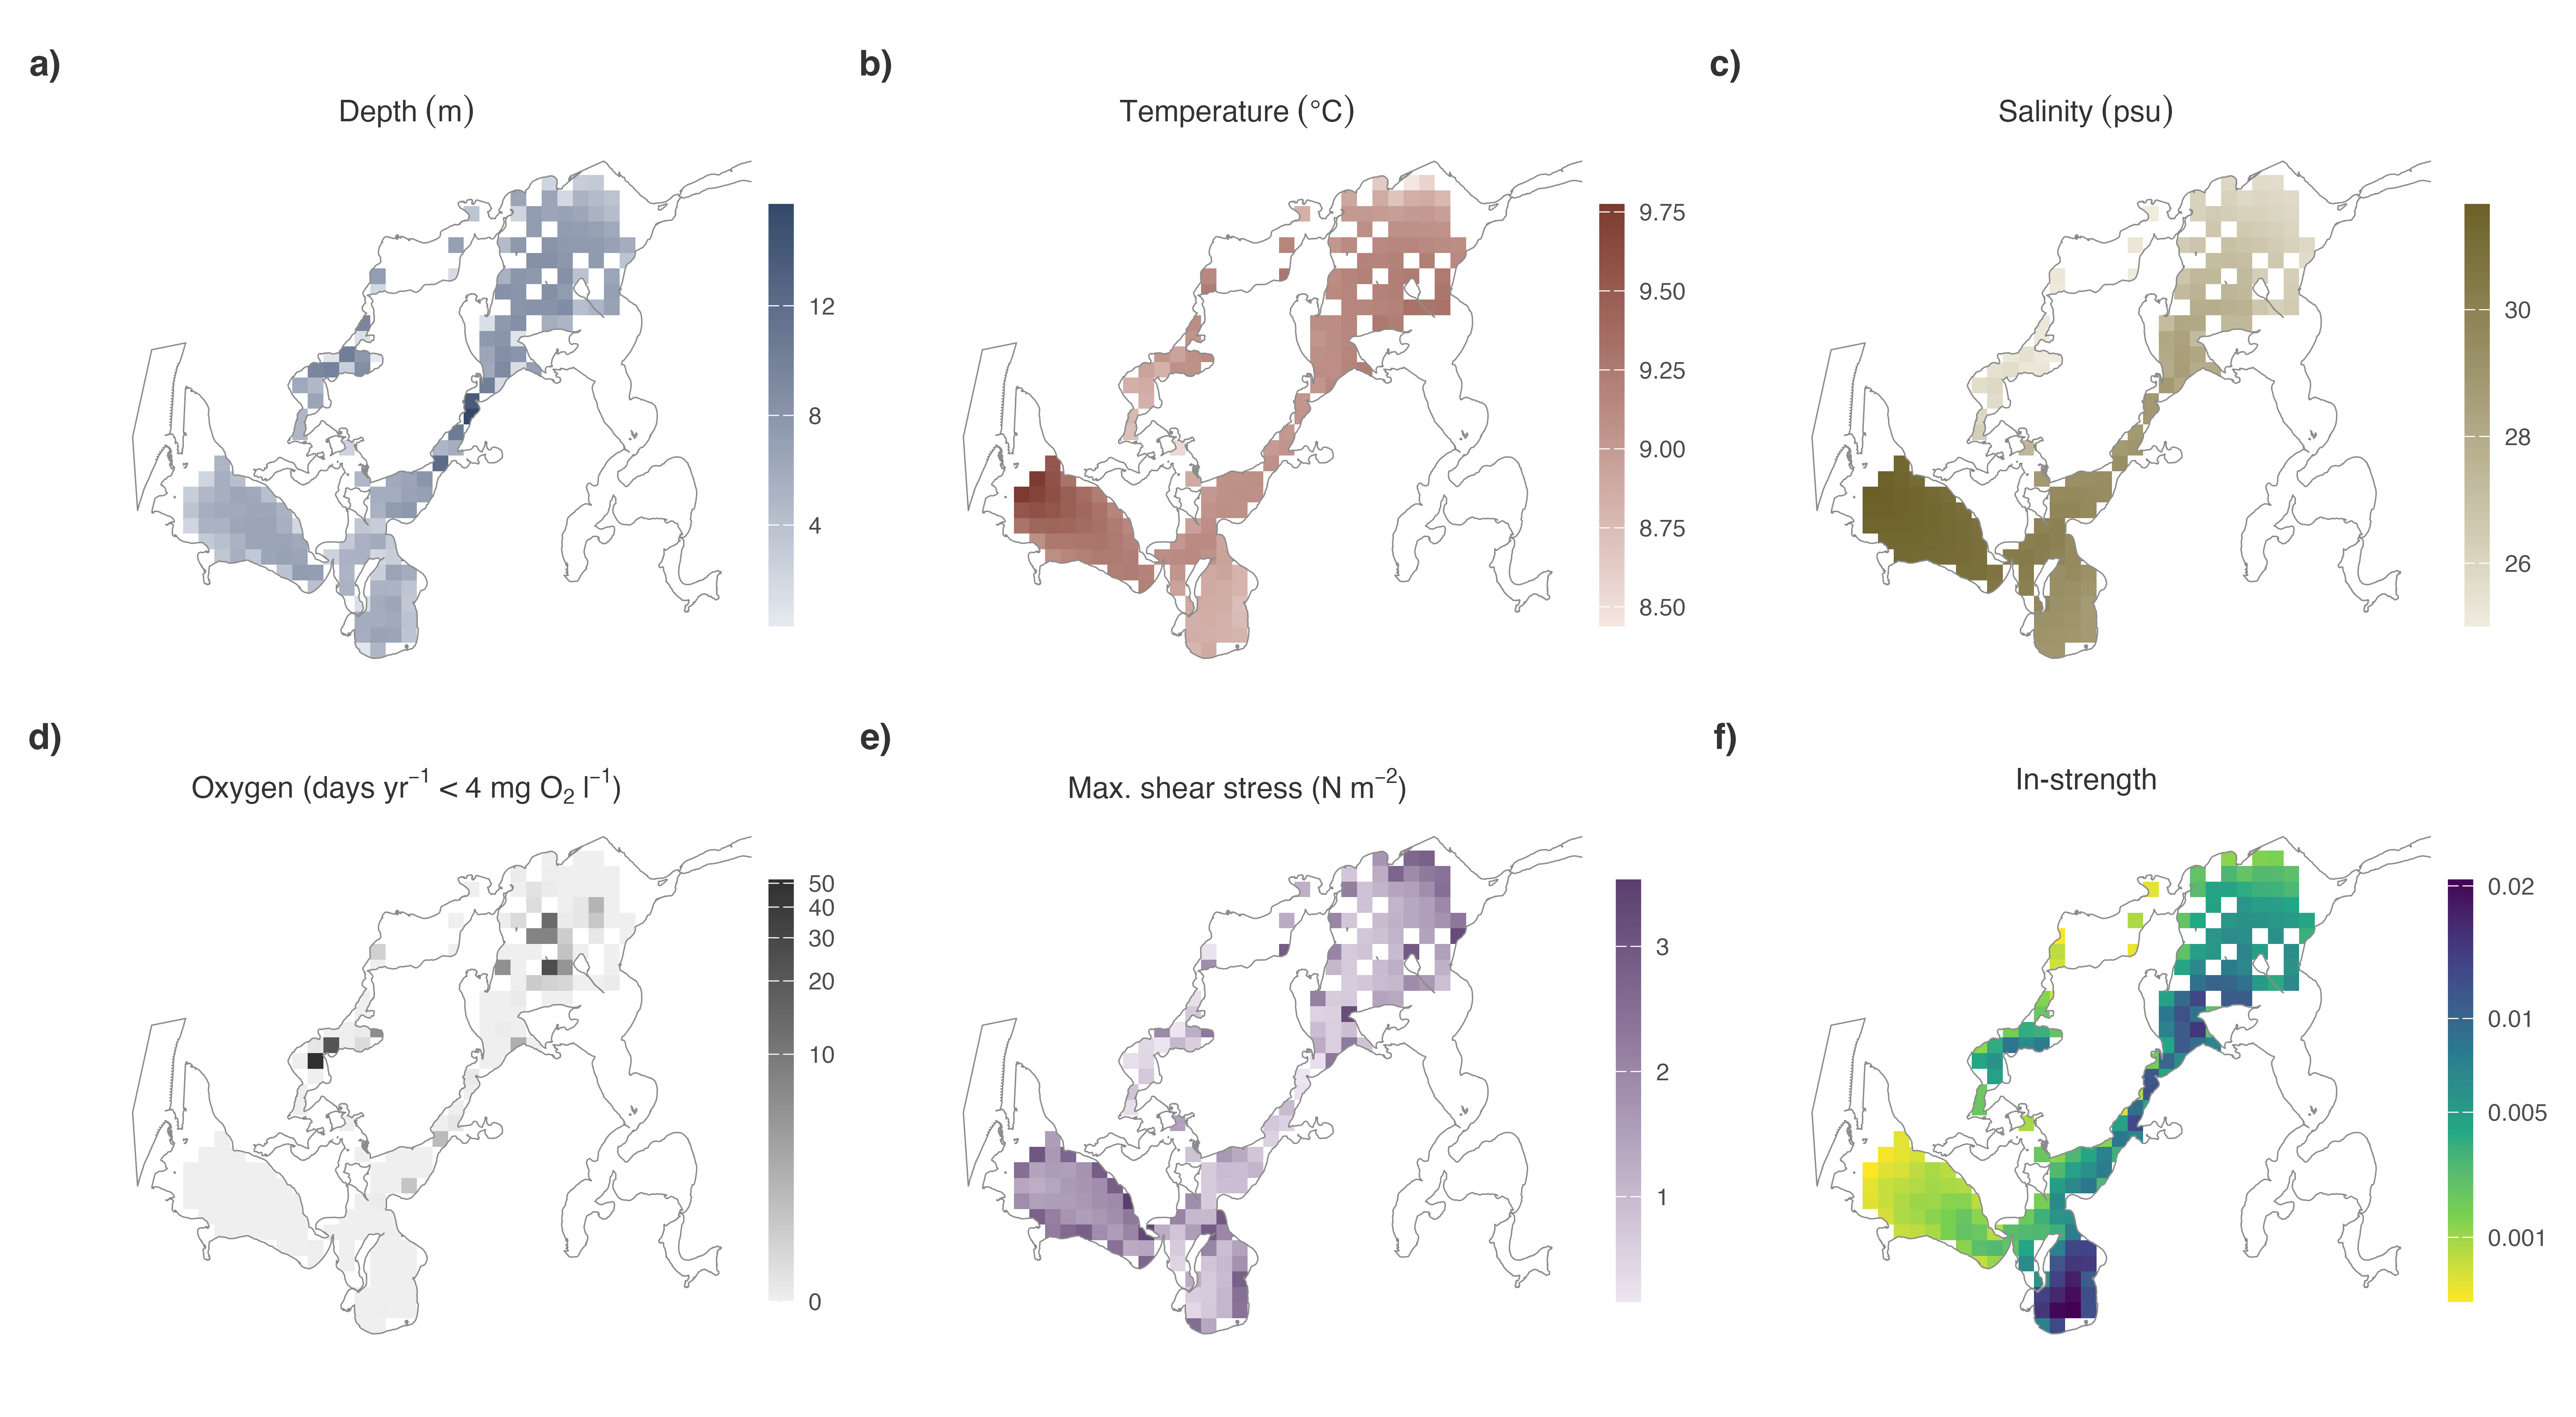
\includegraphics[width=0.95\textwidth]{fig2_predictors.png}
    \caption{\rev{Model predictors at the 2~$\times$~2~km grid cells containing at least one survey station: (a) depth, (b) bottom temperature, (c) bottom salinity, (d) oxygen (days per year with bottom dissolved oxygen below 4~mg~l$^{-1}$), (e) maximum bottom shear stress, and (f) presence-weighted in-strength, the connectivity metric used in the models.}}
    \label{fig:predictors}
\end{figure}

\rev{Because no single connectivity metric was assumed to best represent larval connectivity, we fitted separate models for each of five candidate connectivity metrics (Fig.~\ref{fig:connectivity_maps}): in-degree, in-strength, in-closeness, eigenvector centrality, and transitivity, replacing the connectivity term ($C_i$) in the linear predictor while keeping all other model components unchanged. Based on the results below, in-strength was used as the primary connectivity metric; the other four are reported as a sensitivity check.}

To assess whether the effects differed between biomass and occurrence, we additionally fitted Bernoulli GLMMs to presence--absence data ($z_i\in\{0,1\}$) using a logit link,
\[
z_i \sim \operatorname{Bernoulli}(\pi_i), \qquad
\operatorname{logit}(\pi_i)=\eta_i,
\]
with the same linear predictor. Results from these models are presented in the Supporting Information.

\subsubsection{Model structures comparison}

To quantify the effect and relative contribution of environmental conditions, larval connectivity, and residual spatial structure, we compared six model structures (Table~\ref{tab:model_structures}), in which the environment ($E$), connectivity ($C$), and spatial random field ($\omega$) were included in different combinations.

\begin{table}[h]

\centering

\caption{\rev{Model structures compared. The connectivity term ($C$) was fitted separately using each of the five candidate connectivity metrics.}}

\label{tab:model_structures}
\begin{tabular}{ll}
\toprule
Structure & Linear predictor \\
\midrule
Space                              & $\beta_0 + \omega$ \\
Environment                        & $\beta_0 + E$ \\
Space + Environment                & $\beta_0 + E + \omega$ \\
Space + Connectivity               & $\beta_0 + C + \omega$ \\
Environment + Connectivity         & $\beta_0 + E + C$ \\
Space + Environment + Connectivity & $\beta_0 + E + C + \omega$ \\
\bottomrule
\end{tabular}
\end{table}

\rev{Models containing the connectivity term ($C$; structures 4--6 in Table~\ref{tab:model_structures}) were fitted separately for each of the five candidate connectivity metrics, yielding $3 + (3 \times 5) = 18$ models per response variable (36 models in total for biomass and presence--absence). As a further robustness check specific to the primary (in-strength) metric, the full Space + Environment + Connectivity structure was also refit with each of the five environmental predictors dropped in turn, with and without the spatial field (20 additional models; see \nameref{sec:connectivity_robustness}), and with flipped in-strength in place of in-strength (2 additional models).} Competing models were compared using Akaike's Information Criterion (AIC; \citet{akaike1974}), with lower AIC values indicating better support after accounting for model complexity.

\subsubsection{Spatial field and mesh}

The random field was approximated by the SPDE method on a finite-element mesh built with the R package \texttt{fmesher} \citep{lindgrenFmesherTriangleMeshes2025}, using a maximum inner triangle edge of 2~km (about half the estimated Mat\'ern range). Because the
Limfjorden is a narrow, branching system in which straight-line distance is a poor proxy for connection through water, we used a barrier mesh where mesh triangles
falling on land had their correlation range reduced to 10\% of the water value, so spatial correlation does not cross land \citep{bakkaNonstationaryGaussianModels2019}.

\subsubsection{Variance partitioning}

To assess the relative importance of predictors we decomposed the variance in cockle biomass following the marginal and conditional $R^2$ framework for GLMMs \citep{nakagawa2013, nakagawa2017}. Working on the link scale, we computed three components: the variance of the fixed-effects linear predictor $\sigma^2_f$, the
variance of the spatial random field $\sigma^2_\omega$, and the observation-level (distribution) variance $\sigma^2_d$. For a Tweedie response with a log link the
last was obtained by the lognormal approximation. Marginal
$R^2 = \sigma^2_f / (\sigma^2_f + \sigma^2_\omega + \sigma^2_d)$ is the share of
variance explained by the fixed effects alone, and conditional
$R^2 = (\sigma^2_f + \sigma^2_\omega) / (\sigma^2_f + \sigma^2_\omega + \sigma^2_d)$
the share explained by the fixed effects and the spatial field together.

\rev{To attribute the fixed-effect share to the environment and connectivity blocks ($\eta^f_i = E_i + C_i$), each block was given a share proportional to its own variance, $\mathrm{Var}(B)$, computed from that block's columns alone (i.e. ignoring its covariance with the other block) and then rescaled so the two block shares summed exactly to the fixed-effect share $\sigma^2_f/(\sigma^2_f+\sigma^2_\omega+\sigma^2_d)$ reported above \citep[following the variance-partitioning approach in the \texttt{Hmsc} package,][]{tikhonovJointSpeciesDistribution2020}. This keeps every block's share non-negative even though environment and connectivity are correlated (Fig.~\ref{fig:conn_environment}); the alternative of splitting by each block's covariance with the whole fixed predictor is an exact decomposition of $\sigma^2_f$ but can assign a block a negative share under collinearity, which we found made it harder to report cleanly for the less stable connectivity metrics (\nameref{sec:connectivity_robustness}).}


\subsubsection{Model fitting}
We fit the spatiotemporal models with the R package \texttt{sdmTMB} \citep{andersonSdmTMBPackageFast2025}, version 0.6.0.9034. sdmTMB uses automatic differentiation and the Laplace approximation from the R package TMB \citep{kristensenTMBAutomaticDifferentiation2016} and sparse matrix structures to set up the SPDE-based GMRFs from the R package fmesher \citep{lindgrenFmesherTriangleMeshes2025}. Estimation is done via maximum marginal likelihood. We confirmed that the nonlinear optimization was consistent with convergence by checking that the Hessian matrix was positive definite and the maximum absolute log-likelihood gradient with respect to fixed effects was <0.001 \citep{andersonSdmTMBPackageFast2025}. 

% ---- RESULTS ---------------------------------------------------------------
\section{Results}

\rev{Throughout the survey domain and time frame considered (Stock survey only, $n=5{,}588$ stations), cockles were present at 23.0\% of stations.} Biomass was concentrated in a few dense beds along the central channel and south-western basins (Fig.~\ref{fig:study_area}a). The biophysical model predicted extensive potential larval exchange throughout the entire area, although settlement remained spatially structured. Depending on release location, 90\% of larvae settled within \rev{324--620}~km$^2$ of the release cell, compared with a connected basin of approximately 2,400 km$^2$ (Fig.~\ref{fig:study_area}b). \textcolor{red}{Not sure about this need help with interpretation @Ane @Flemming}

\begin{figure}[htbp]
    \centering
    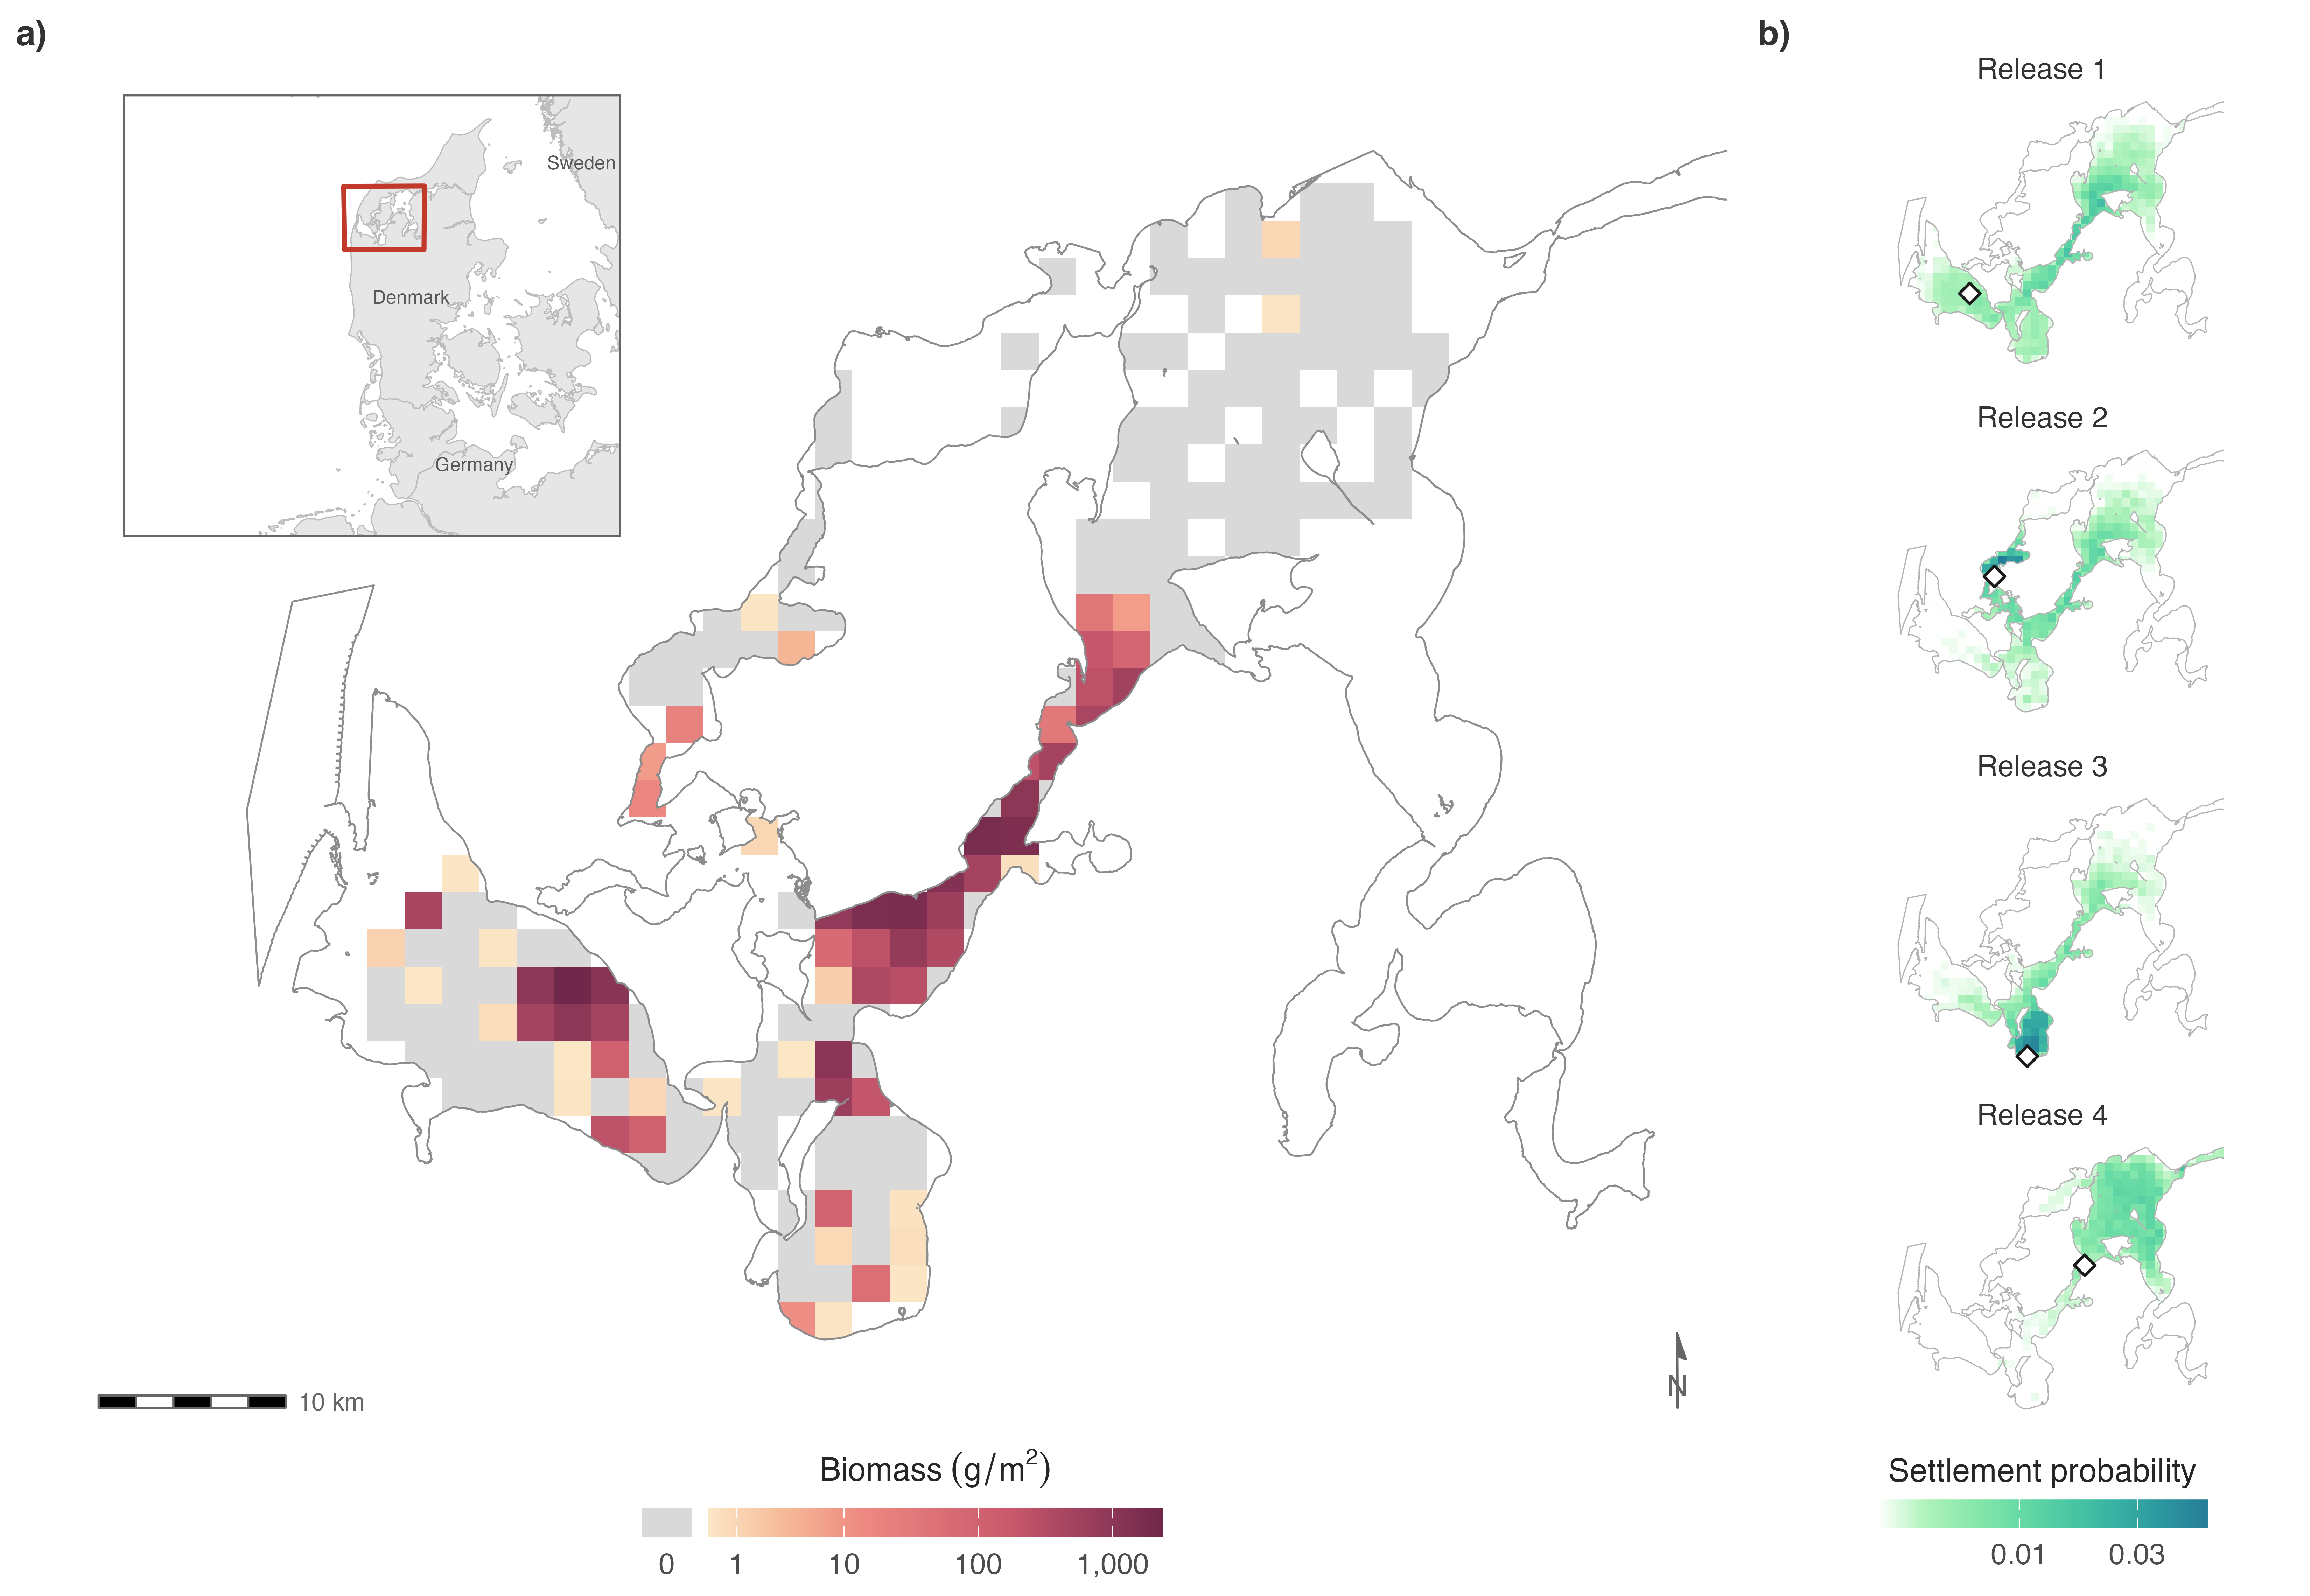
\includegraphics[width=0.95\textwidth]{fig1_map.png}
    \caption{\rev{(a) Study area. Mean cockle biomass density in each 2~$\times$~2~km grid cell containing survey stations in the Limfjorden, Denmark, averaged over all stations and years in the cell; grey cells are those where no cockles were recorded. Inset: location of the Limfjorden. (b) Examples of larval settlement footprints: for each of four release cells (white diamonds), chosen among cells where cockles were recorded, the probability that a released larva settles in each grid cell.}}
    \label{fig:study_area}
\end{figure}


\subsection{Model selection}

\rev{Model selection strongly supported the inclusion of the spatial random field and environmental predictors, whereas support for the connectivity term was comparatively weak (Table~\ref{tab:model-selection}). Relative to the best-supported model (Space + Environment + Connectivity, in-strength), removing the spatial random field increased AIC by $\approx$1,120 units, removing the environmental block increased AIC by $\approx$86 units, and removing the connectivity term increased AIC by only $\approx$8 units ($\approx$4 units for presence--absence). The same ranking of model structures was obtained for the presence--absence models. Among models including environmental predictors, the spatial random field, and connectivity, in-strength and in-closeness fitted almost equally well (in-closeness 1.4 AIC units lower for biomass and 0.1 lower for presence--absence), and the remaining metrics were within 8.4 AIC units of in-strength (eigenvector centrality +2.2, in-degree +4.1, transitivity +8.4 for biomass), indicating little evidence that one connectivity metric outperformed the others on fit alone. In-strength was carried forward as the primary metric because, unlike the other four, its coefficient kept its sign and significance with and without the spatial field in both responses (\nameref{sec:connectivity_robustness}); the other four are reported there as a sensitivity comparison.}

\begin{table}[ht]
\centering
\small
\caption{Model selection for cockle presence, biomass where present and both together (the delta-gamma model). $\Delta$AIC is the difference in AIC to the best model (lower AIC is better). $\Delta$ELPD is the difference in expected log predictive density to the best model in spatially blocked 10-fold cross-validation (higher ELPD is better), with its standard error in parentheses. The best model in each column is shown in bold. The total AIC and ELPD are the sums of the two parts. All models include survey (gear) and year as factors and a spatial random field. Connectivity is presence-weighted in-strength; environment comprises depth (linear and quadratic), temperature, oxygen, salinity, and maximum shear stress. A dash marks a model that did not converge.}
\label{tab:model-selection}
\begin{tabular}{lrrrrrr}
\toprule
 & \multicolumn{3}{c}{$\Delta$AIC} & \multicolumn{3}{c}{$\Delta$ELPD (SE)} \\
\cmidrule(lr){2-4} \cmidrule(lr){5-7}
Model & Presence & Biomass & Total & Presence & Biomass & Total \\
\midrule
Space + Environment & 1.8 & 1.6 & \textbf{0.0} & -18.8 (4.6) & -51.9 (32.9) & -33.7 (24.7) \\
Space + Environment + Connectivity & \textbf{0.0} & 3.5 & 0.1 & \textbf{0.0} & -37.0 (10.9) & \textbf{0.0} \\
Space & 62.8 & \textbf{0.0} & 59.3 & -87.2 (10.9) & \textbf{0.0} & -50.2 (15.6) \\
Space + Connectivity & 63.8 & 1.9 & 62.2 & -93.9 (10.7) & -50.4 (29.7) & -107.2 (24.9) \\
\bottomrule
\end{tabular}
\end{table}



\subsection{Effects of habitat, connectivity and space}

\rev{Cockles were most abundant in shallow, low-energy water (Fig.~\ref{fig:coefficients}a). The fitted responses show that biomass declined with depth ($\hat{\beta}=-1.05\pm0.15$ per SD) and maximum shear stress ($-1.28\pm0.16$); salinity ($0.71\pm0.44$), oxygen ($-0.27\pm0.21$) and temperature ($0.21\pm0.51$) were not distinguishable from zero at the 95\% level. The presence--absence model gave the same picture for depth ($-0.79\pm0.13$) and shear stress ($-1.22\pm0.16$), with salinity additionally positive ($0.46\pm0.21$). This is a change from an earlier version of this analysis that also included the Commercial survey, in which salinity and oxygen were significant -- dropping Commercial (see Methods) both removed $\approx$1,900 rows and removed the survey/gear term, and the wider confidence intervals here reflect that. Beyond these environmental gradients, residual spatial autocorrelation decayed over a Mat\'ern range of 3.9 km, corresponding to about two grid cells.}

\rev{The in-strength coefficient was negative for both responses (biomass: $-0.35\pm0.11$; presence: $-0.28\pm0.11$; Fig.~\ref{fig:coefficients}a), so cells receiving more modelled larval supply held less cockle biomass and were less likely to have cockles present, all else equal. For biomass, in-degree, in-closeness and eigenvector centrality were also negative with 95\% CIs excluding zero, while transitivity was positive but not distinguishable from zero; for presence, only in-strength and in-closeness had CIs excluding zero (\nameref{sec:connectivity_robustness}).}

\begin{figure}[htbp]
    \centering
    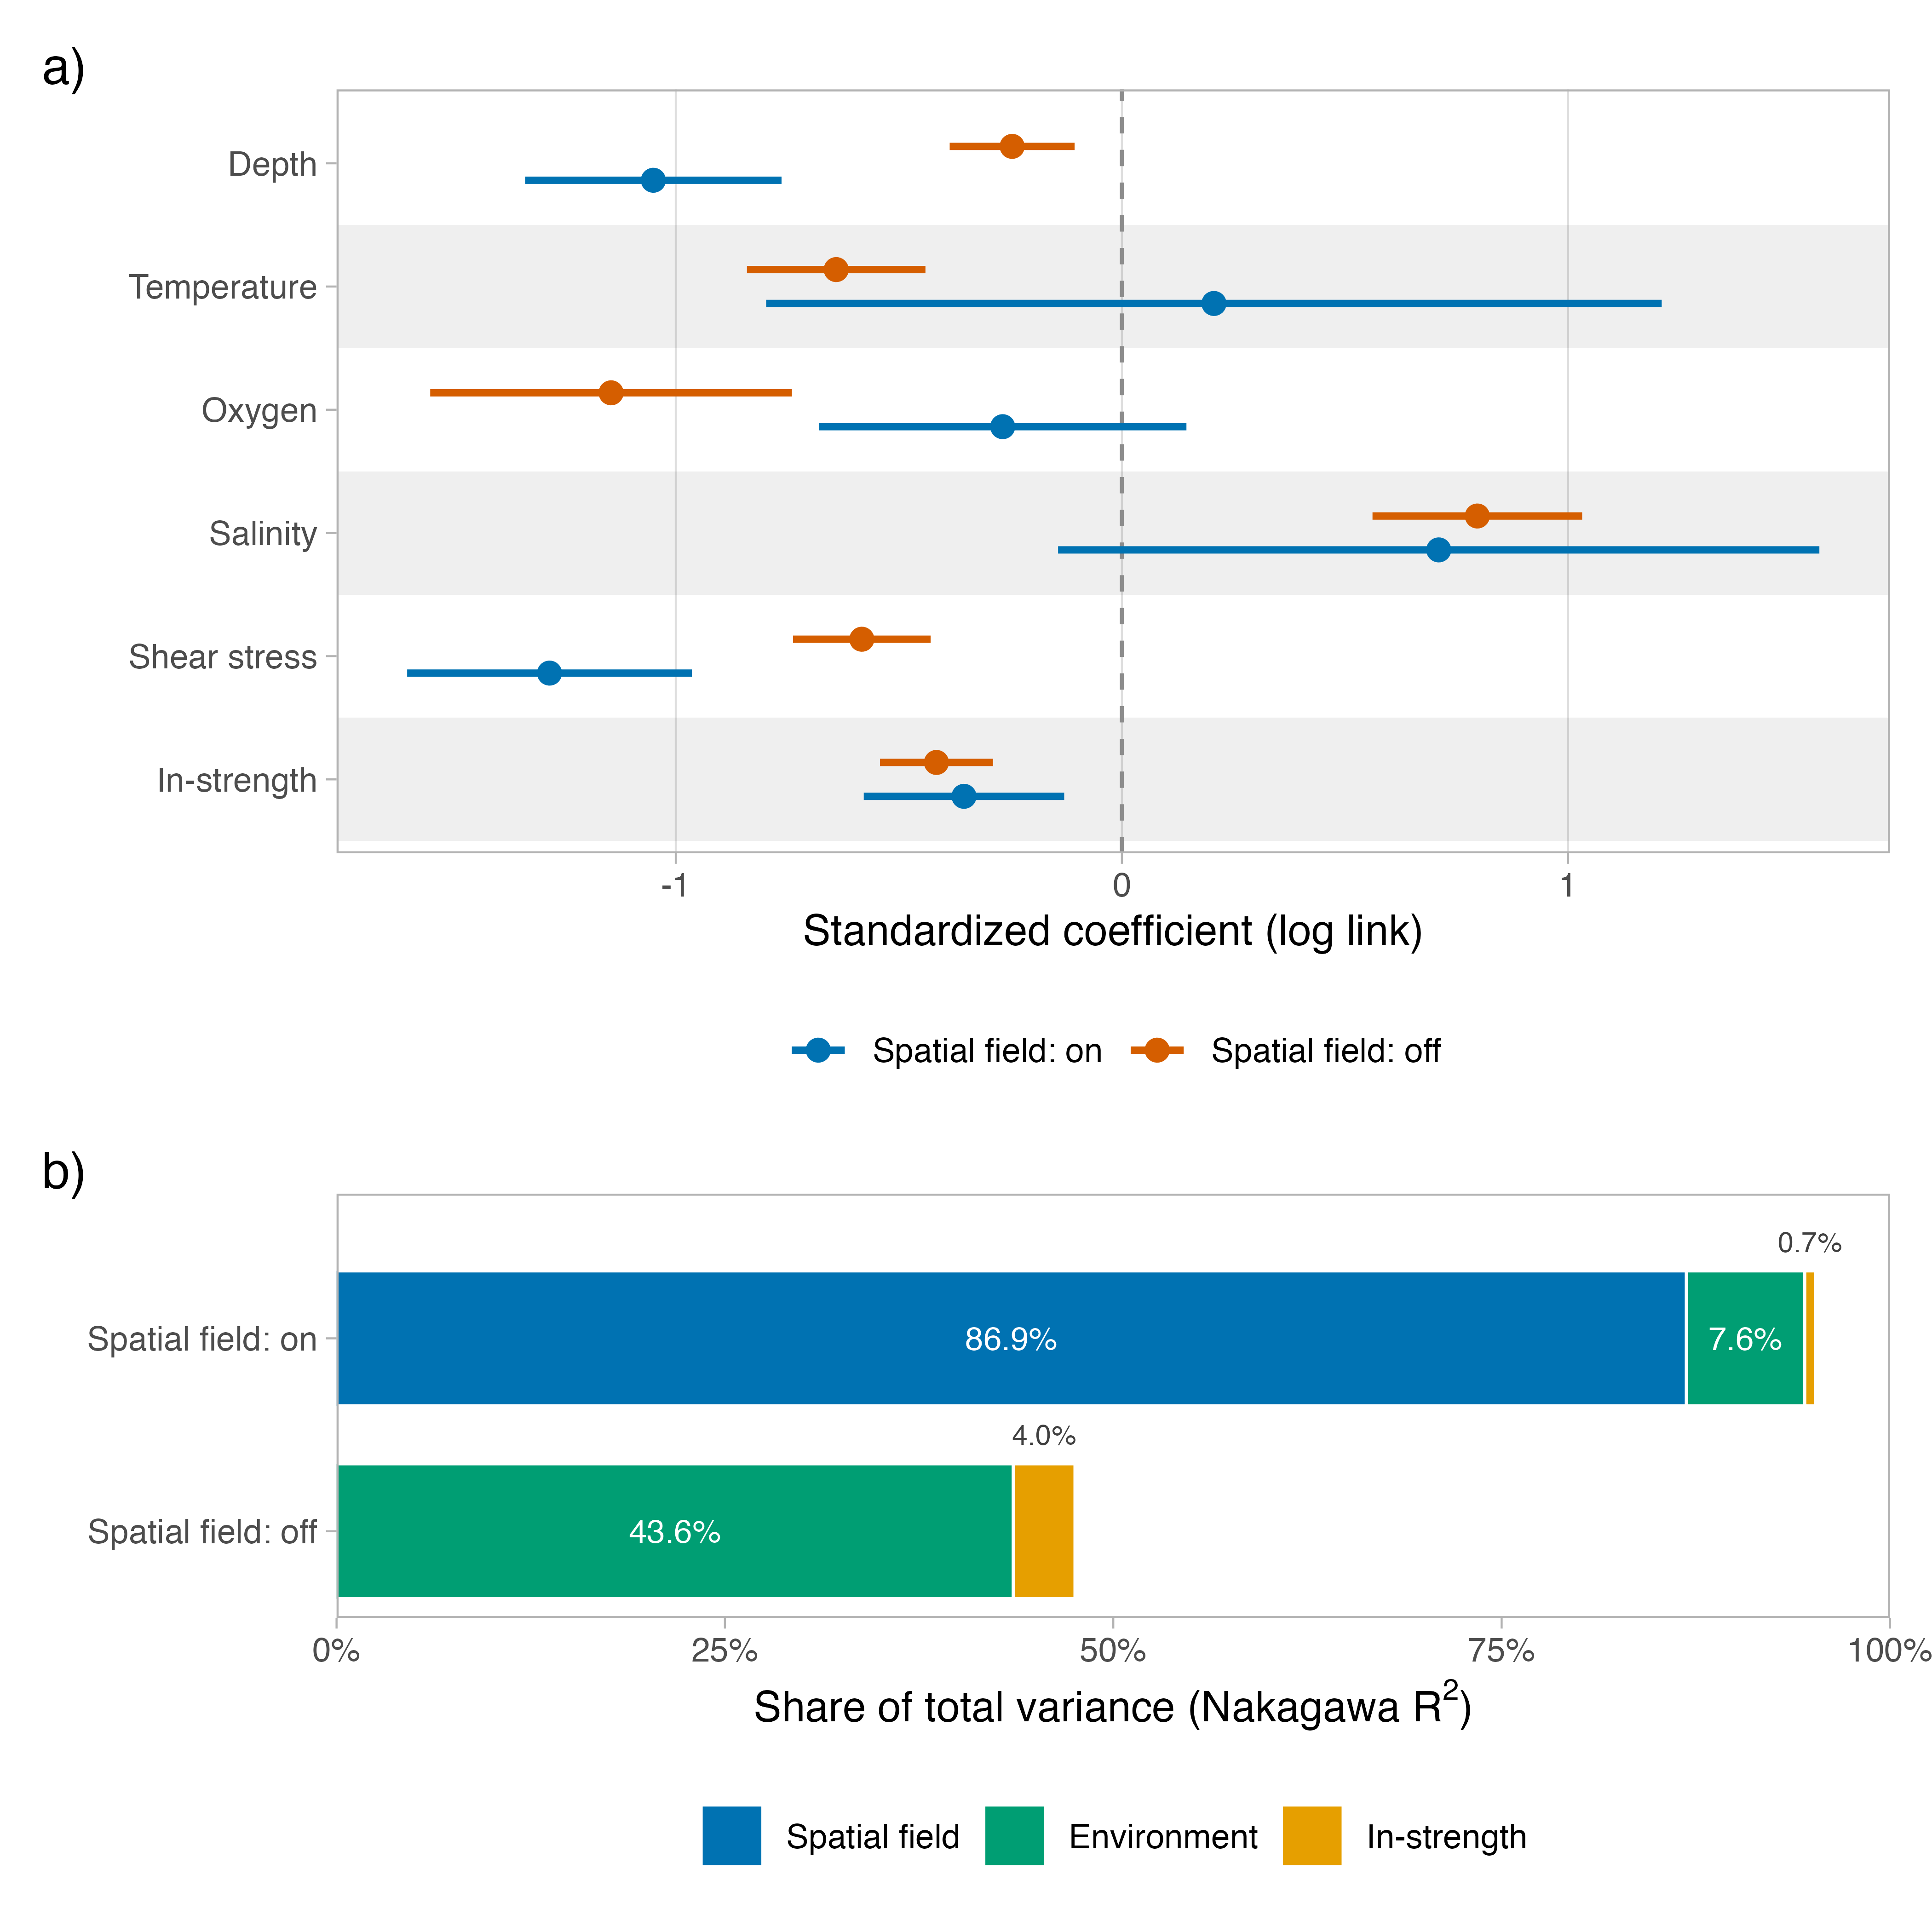
\includegraphics[width=0.95\textwidth]{fig3_coeff.png}
    \caption{\rev{Full Space + Environment + Connectivity biomass density model (Tweedie, log link), presence-weighted in-strength as the connectivity metric, with and without the spatial random field. (a) Standardized coefficients with 95\% confidence intervals. (b) Variance partitioning (Nakagawa marginal/conditional $R^2$; fixed-effect blocks split as described in Methods); the remainder of each bar to 100\% is unexplained (observation-level) variance. The presence--absence counterpart is Fig.~\ref{fig:coefficients_presence}.}}
    \label{fig:coefficients}
\end{figure}

\rev{Variance partitioning was consistent with the AIC-based model selection (Fig.~\ref{fig:coefficients}b). With the spatial field included, it accounted for 86.9\% of the total variance in biomass, followed by the environment (7.6\%) and connectivity (0.7\%), leaving 4.8\% unexplained; for presence the corresponding shares were 59.5\% (space), 10.8\% (environment), 0.6\% (connectivity) and 29.1\% unexplained. Replacing in-strength with each of the other four connectivity metrics gave a similar picture (Fig.~\ref{fig:variance_metrics}): with the field included, connectivity's share ranged 0.5--2.3\% for biomass and 0.4--1.2\% for presence, while the spatial field's share stayed within 86.5--87.9\% (biomass) and 58.9--60.6\% (presence) regardless of which metric was used.}

\subsection{Connectivity relative to habitat and spatial structure}
\label{sec:connectivity_robustness}

\rev{The five connectivity metrics correlated with the environmental predictors to varying degrees (Fig.~\ref{fig:conn_spatial}). For in-degree, in-strength, in-closeness and eigenvector centrality, Spearman correlations ranged $\rho=0.48$ to $0.62$ with depth, $-0.28$ to $-0.83$ with salinity, $-0.43$ to $-0.62$ with maximum shear stress, and $0.22$ to $0.36$ with oxygen. Transitivity correlated with the same variables but with the \emph{opposite} sign ($\rho=-0.32$ with depth, $+0.42$ with salinity, $+0.55$ with maximum shear stress), consistent with transitivity behaving as an inverse measure of network centrality: hub-like cells with many connections tend to have low clustering. In-degree and in-closeness were themselves almost collinear ($\rho=0.98$; Fig.~\ref{fig:conn_environment}), so the five metrics represent closer to three or four independent pieces of information than five. None of the metrics tracked the residual spatial structure: their correlation with the spatial random field of the Space + Environment model was weak ($|\rho|\le0.21$), and essentially zero for in-strength ($\rho=0.01$).}

\rev{Refitting each connectivity model without the spatial field moved the five metrics very differently (Fig.~\ref{fig:space_confounding}). In-strength was the most stable: its coefficient barely moved (biomass $-0.35\rightarrow-0.42$; presence $-0.28\rightarrow-0.39$), and it was the only metric whose sign and significance were unchanged in both responses. In-degree flipped sign in both responses when the field was dropped (biomass $-0.58\rightarrow+0.64$; presence $-0.34\rightarrow+0.24$), and in-closeness lost its effect (biomass $-0.64\rightarrow+0.13$; presence $-0.41\rightarrow-0.04$); eigenvector centrality kept its sign but was not distinguishable from zero for presence with the field included, and transitivity was not distinguishable from zero with the field included in either response. As a further check specific to in-strength, we refit the full model dropping one environmental predictor at a time, with and without the spatial field (20 models, all converged; Fig.~\ref{fig:loo_stability}). The in-strength coefficient stayed within $-0.26$ to $-0.50$ across every combination and its CI excluded zero in all 20 specifications. Dropping depth moved the estimate further from zero and dropping shear stress moved it toward zero; depth, salinity and shear stress are the three covariates most correlated with in-strength above, but the size of a predictor's raw correlation with in-strength did not cleanly predict the size of its leave-one-out shift. None of the 20 specifications reversed the sign.} \ml{Exploratory check, not yet in the text (R/exploration/check\_instrength\_outliers.R): refitting the full model without the survey stations in the high-inflow hub cells of the raw network, or in the top 10\% of cells by in-strength, made the effect stronger rather than weaker (biomass $-0.35\rightarrow-0.64$ and $-0.63$; presence $-0.28\rightarrow-0.54$ and $-0.59$), so the negative effect is not driven by a few extreme cells. Worth adding as a robustness result.}

\rev{Reversing the direction of the network changed the result for presence but not for biomass. With flipped in-strength in place of in-strength, the biomass model fitted equally well ($\Delta$AIC $=-0.7$) and the coefficient remained negative ($-0.22\pm0.07$), whereas the presence--absence model fitted worse ($\Delta$AIC $=+4.3$) and the coefficient was no longer distinguishable from zero ($-0.11\pm0.08$).} \ml{Caution when interpreting this as a pure direction effect: because each source row is weighted by its own presence probability, a cell's flipped in-strength is its export weighted by its \emph{own} modelled presence, which comes from the spatial-field-only suitability model. This is why flipped in-strength correlates with the residual spatial field ($\rho=0.58$) and positively with raw biomass ($\rho=0.28$), unlike in-strength. A cleaner direction test would weight the flipped matrix by destination rather than source presence.}

\rev{Connectivity had almost no marginal association with cockle biomass. Station-level Spearman correlations were $\rho=-0.12$ for in-strength, $-0.09$ for eigenvector centrality and $|\rho|\le0.03$ for in-degree, in-closeness and transitivity. The negative coefficients reported above therefore appear only after conditioning on the environmental covariates and the spatial field, and describe a partial rather than an overall association.}

% ---- DISCUSSION ------------------------------------------------------------
\section{Discussion}


% ---- BACK MATTER -----------------------------------------------------------
\section*{Acknowledgements}
@ Pedro
@ Flemming
@ Martin

\section*{Author contributions}

\section*{Conflicts of interest}
The authors declare that they have no conflict of interest.

\section*{Data Availability Statement}
Code and data are available at \url{https://github.com/user/repo} and archived
at \url{https://doi.org/xxxxx}.

\section*{Funding}
@ Pedro

\bibliography{bib}

\end{spacing}
\clearpage

% ============================================================================
%  TABLES
% ============================================================================
%\section{Tables}

% Both tables are generated by the R pipeline and \input verbatim, so they never
% drift from the fitted models:
%   ../output/tables/tab1_model_selection.tex  <- R/tab1_model_selection.R
% Label: tab:model-selection
% The variance partitioning is shown as Fig.~\ref{fig:variance} rather than a
% table, so tab2 is no longer input here.




\clearpage

% ============================================================================
%  FIGURES
% ============================================================================
% ============================================================================
%  SUPPORTING INFORMATION
%  Figures/tables are relabelled S1, S2, ... and page/line counters reset.
% ============================================================================
\renewcommand{\thetable}{S\arabic{table}}
\setcounter{table}{0}
\renewcommand{\thefigure}{S\arabic{figure}}
\setcounter{figure}{0}
\addtocontents{toc}{\protect\setcounter{tocdepth}{0}}
\renewcommand{\theHfigure}{S\arabic{figure}}
\renewcommand{\theHtable}{S\arabic{table}}
\onehalfspacing
\resetlinenumber
\setcounter{page}{1}
\setcounter{equation}{0}
\nolinenumbers

%\begin{Center}
%\section*{Supporting Information}
%\end{Center}

%\begin{figure}[htb]
%    \centering
%    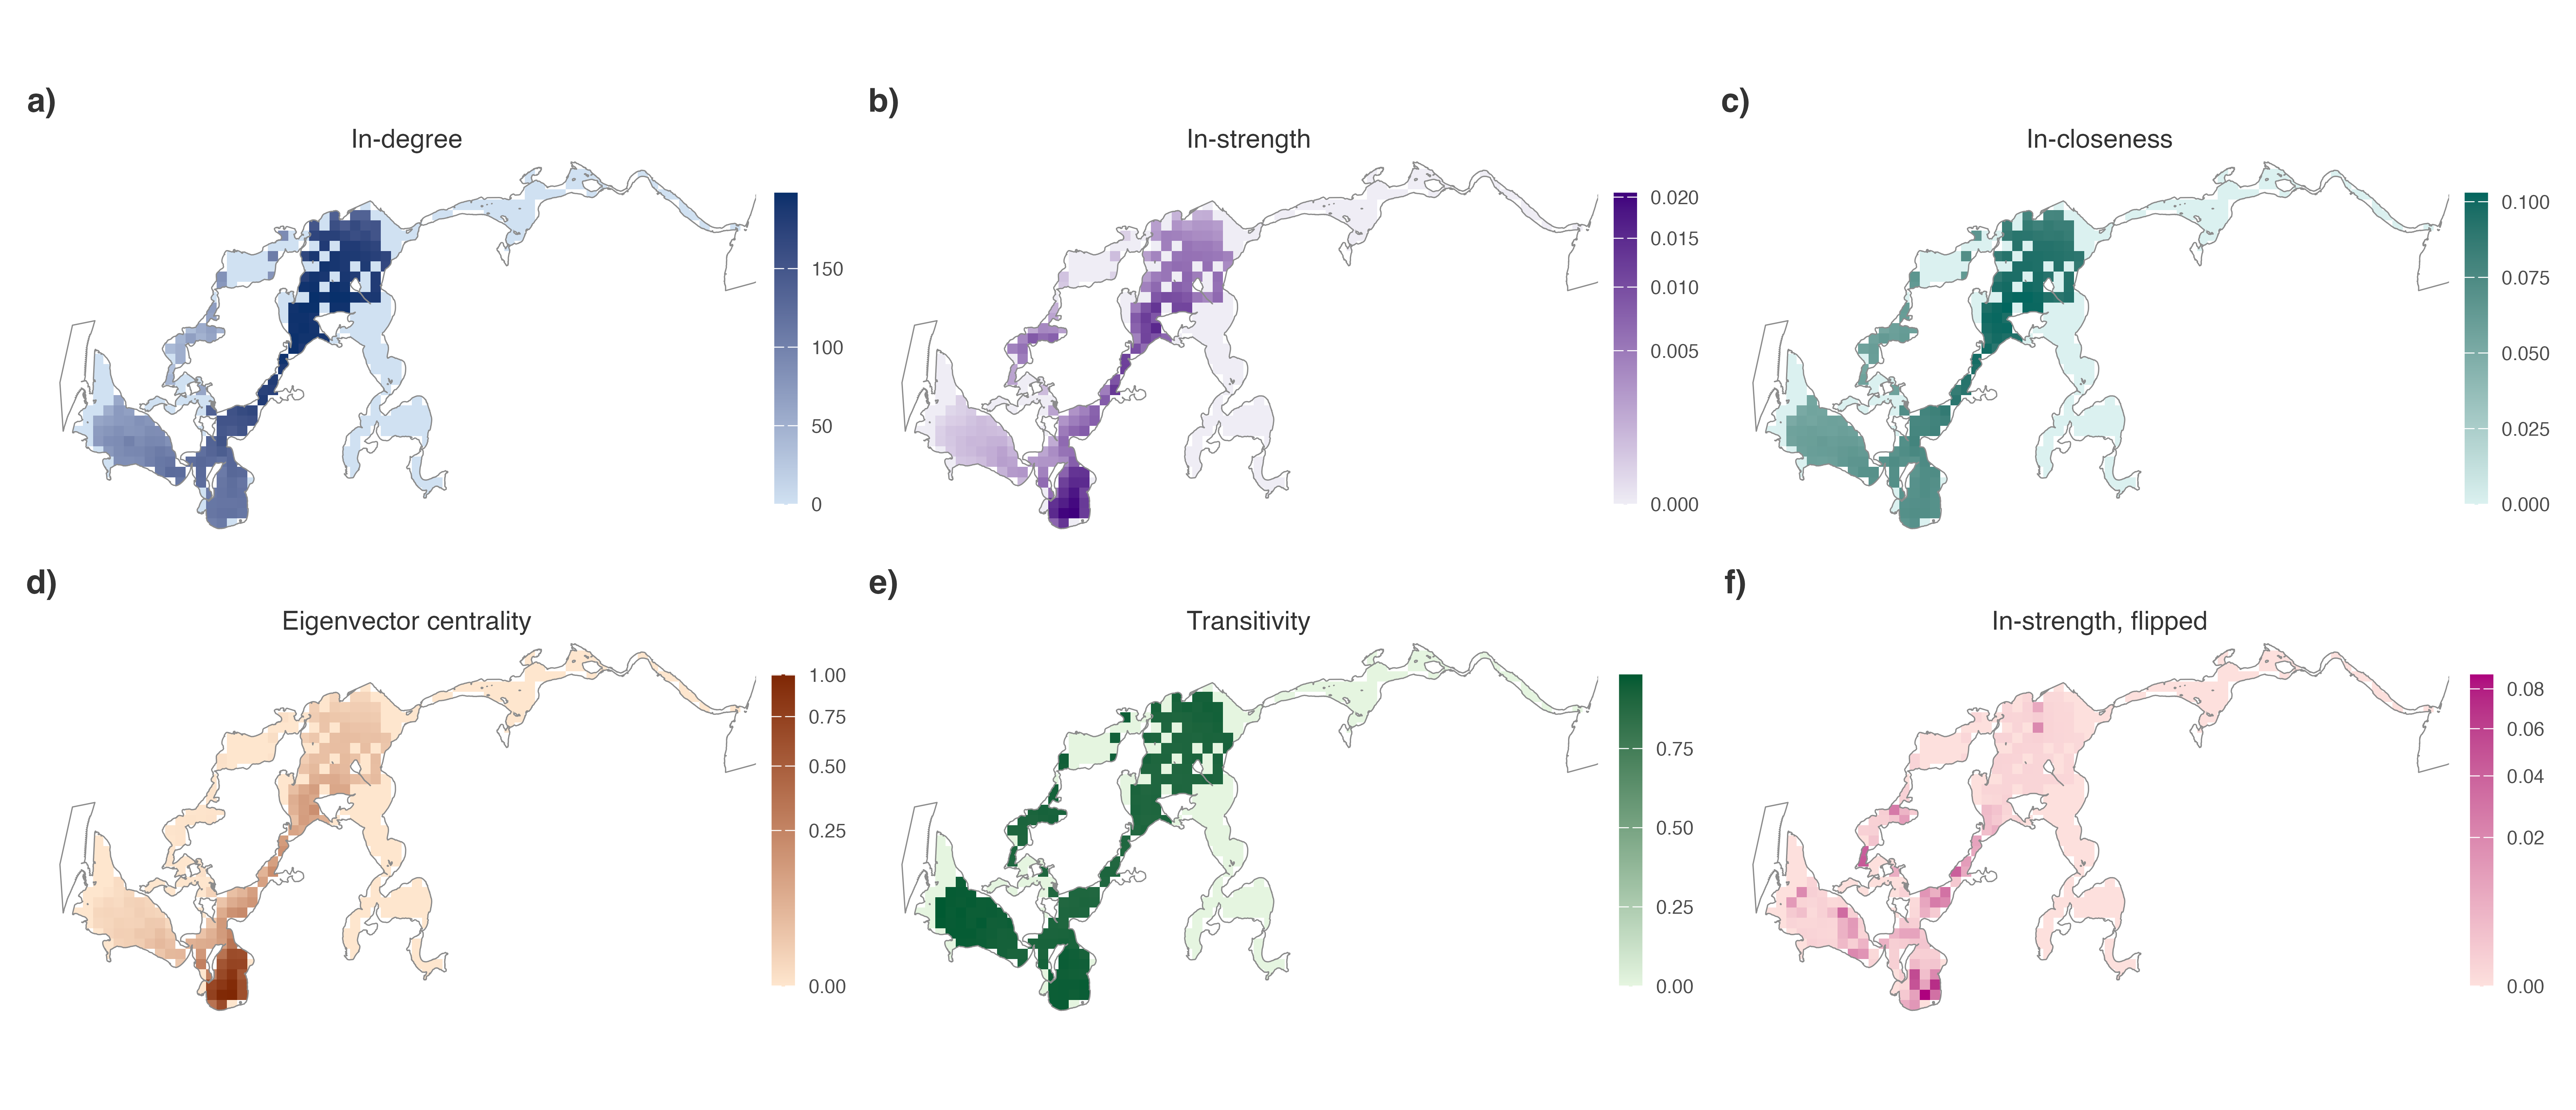
\includegraphics[width=0.95\textwidth]{figS1_connectivity_metrics.png}
%    \caption{\rev{Presence-weighted connectivity metrics mapped on the 2$\times$2~km grid: (a) in-degree, (b) in-strength, (c) in-closeness, (d) eigenvector centrality, (e) transitivity and (f) flipped in-strength (in-strength on the reversed network).}}
%    \label{fig:connectivity_maps}
%\end{figure}
%\FloatBarrier
%\clearpage

%\begin{figure}[htb]
%    \centering
%    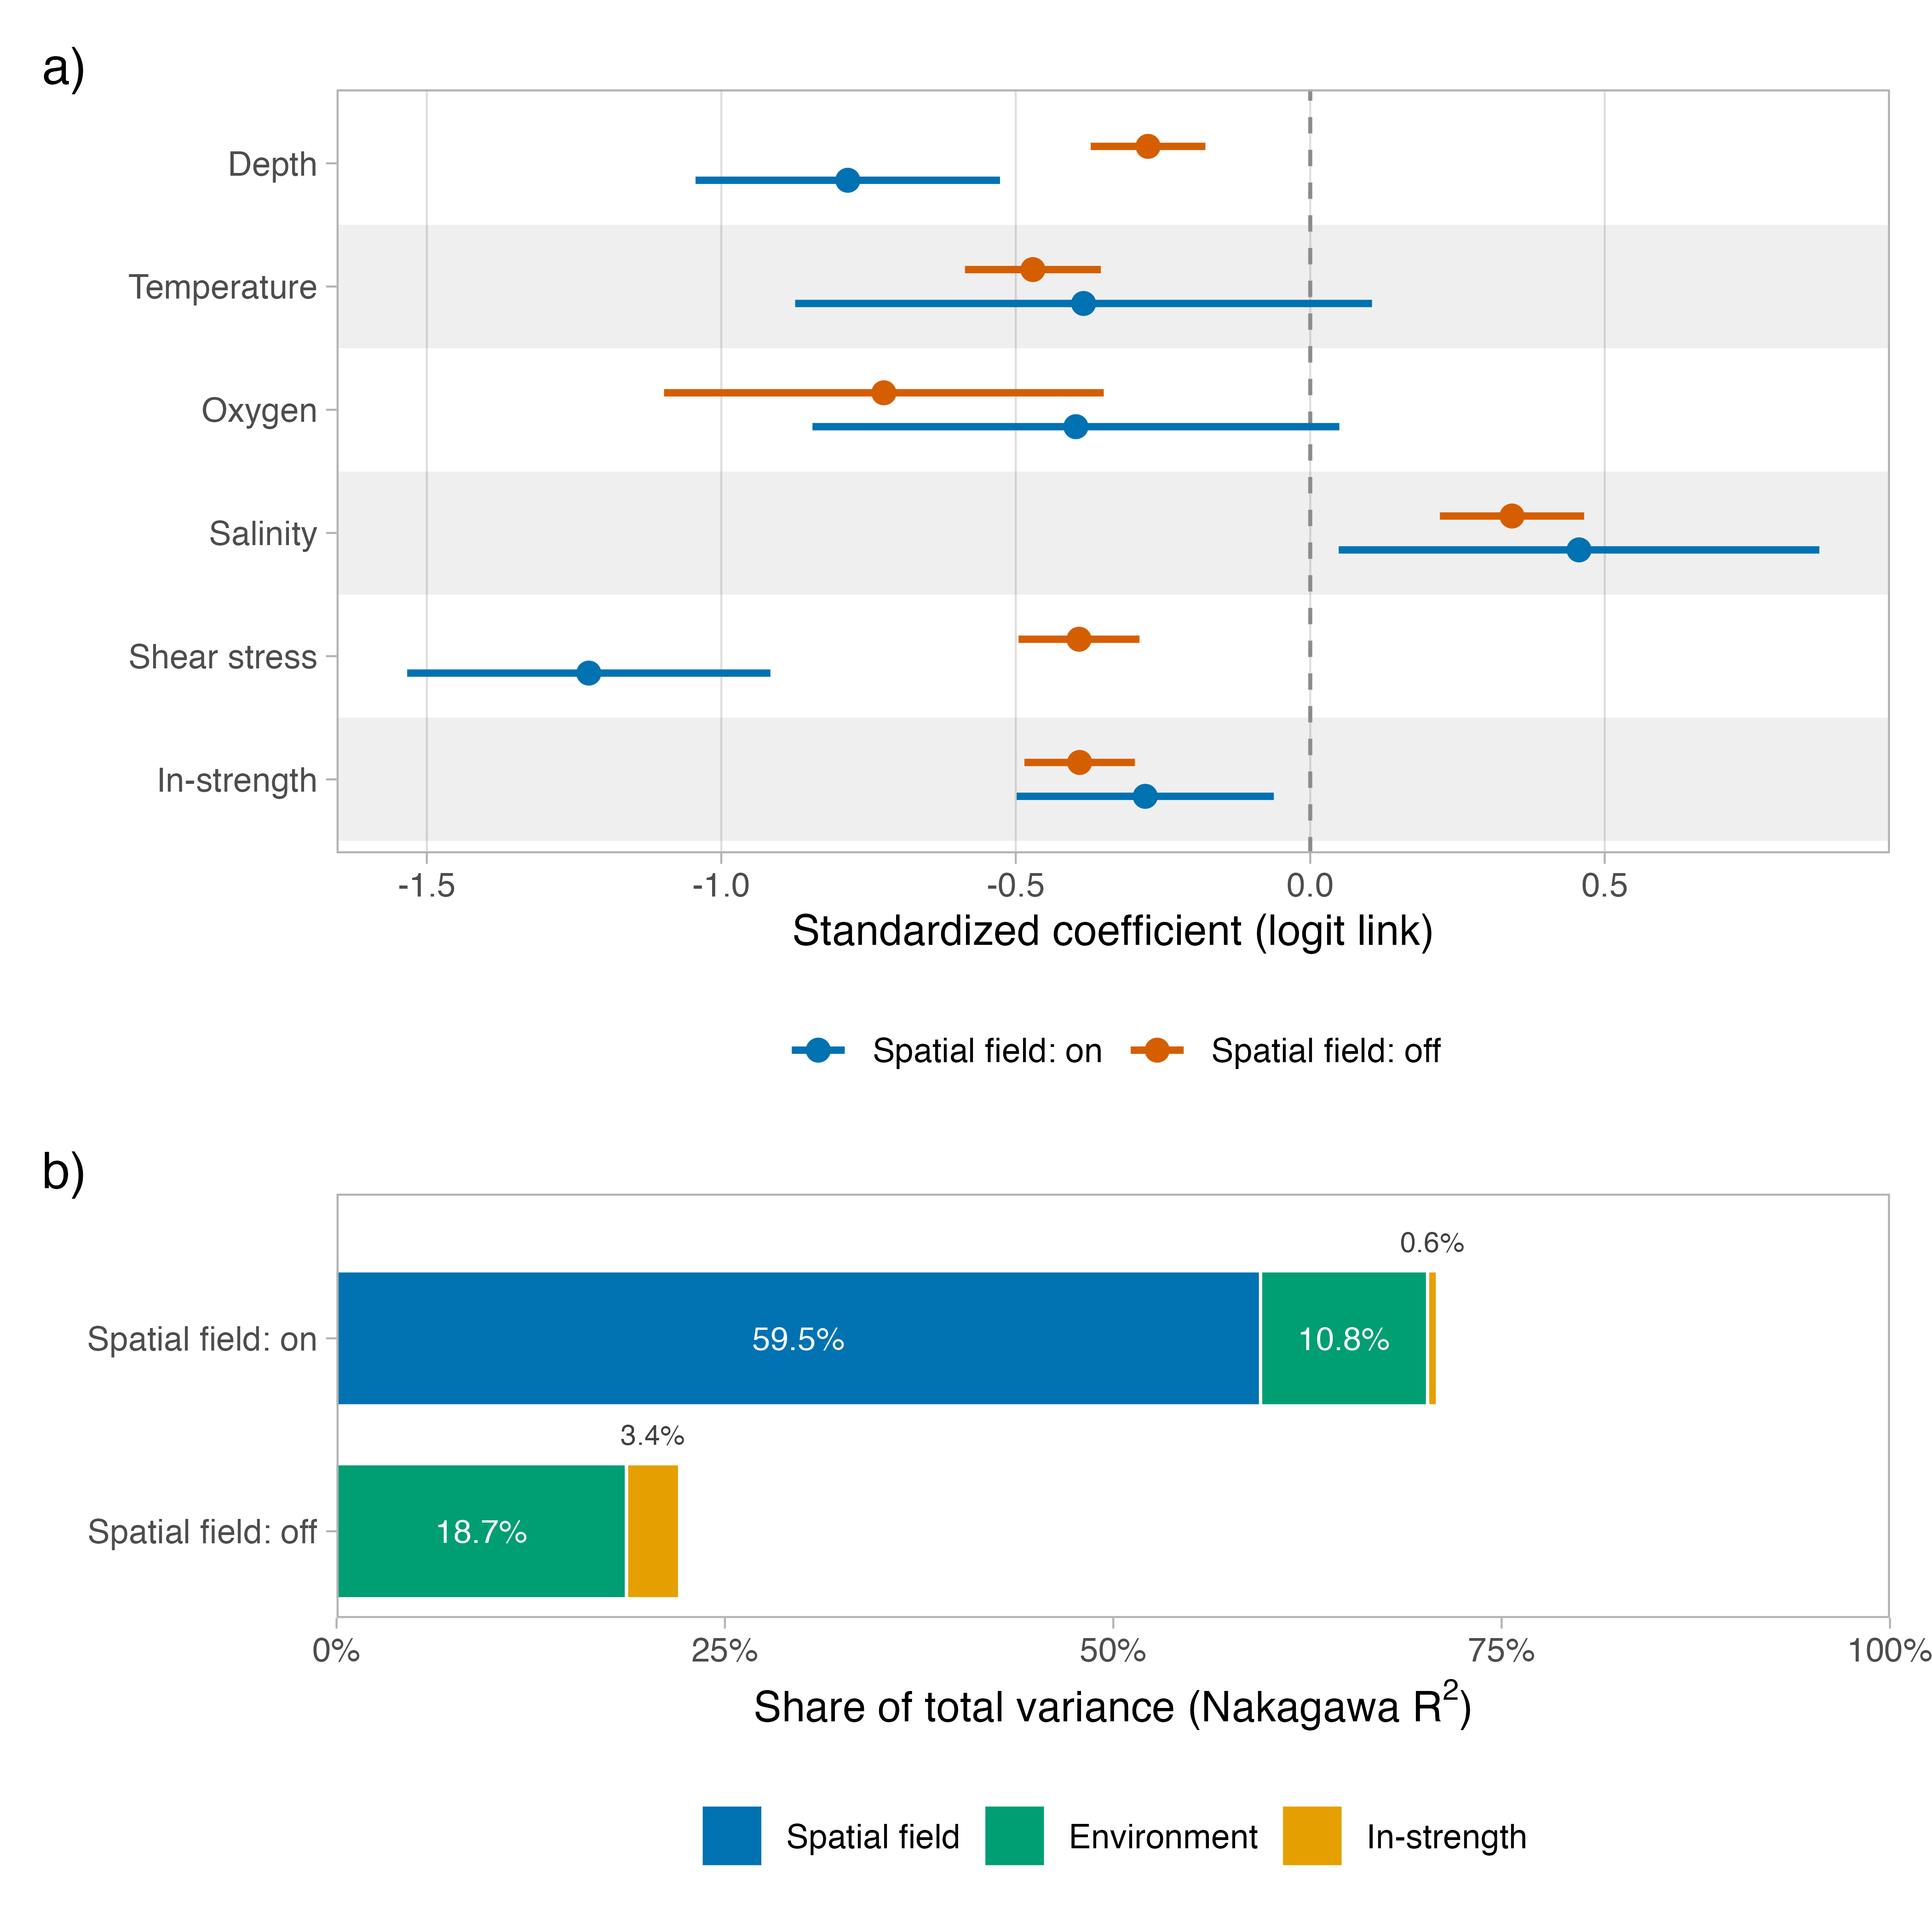
\includegraphics[width=0.95\textwidth]{figS2_coeff_presence.png}
%    \caption{\rev{Full Space + Environment + Connectivity presence model (Bernoulli, logit link), in-strength as the connectivity metric, with and without the spatial random field. (a) Standardized coefficients. (b) Variance partitioning. Counterpart to Fig.~\ref{fig:coefficients}.}}
 %   \label{fig:coefficients_presence}
%\end{figure}
%\FloatBarrier
%\clearpage

%\begin{figure}[htb]
 %   \centering
  %  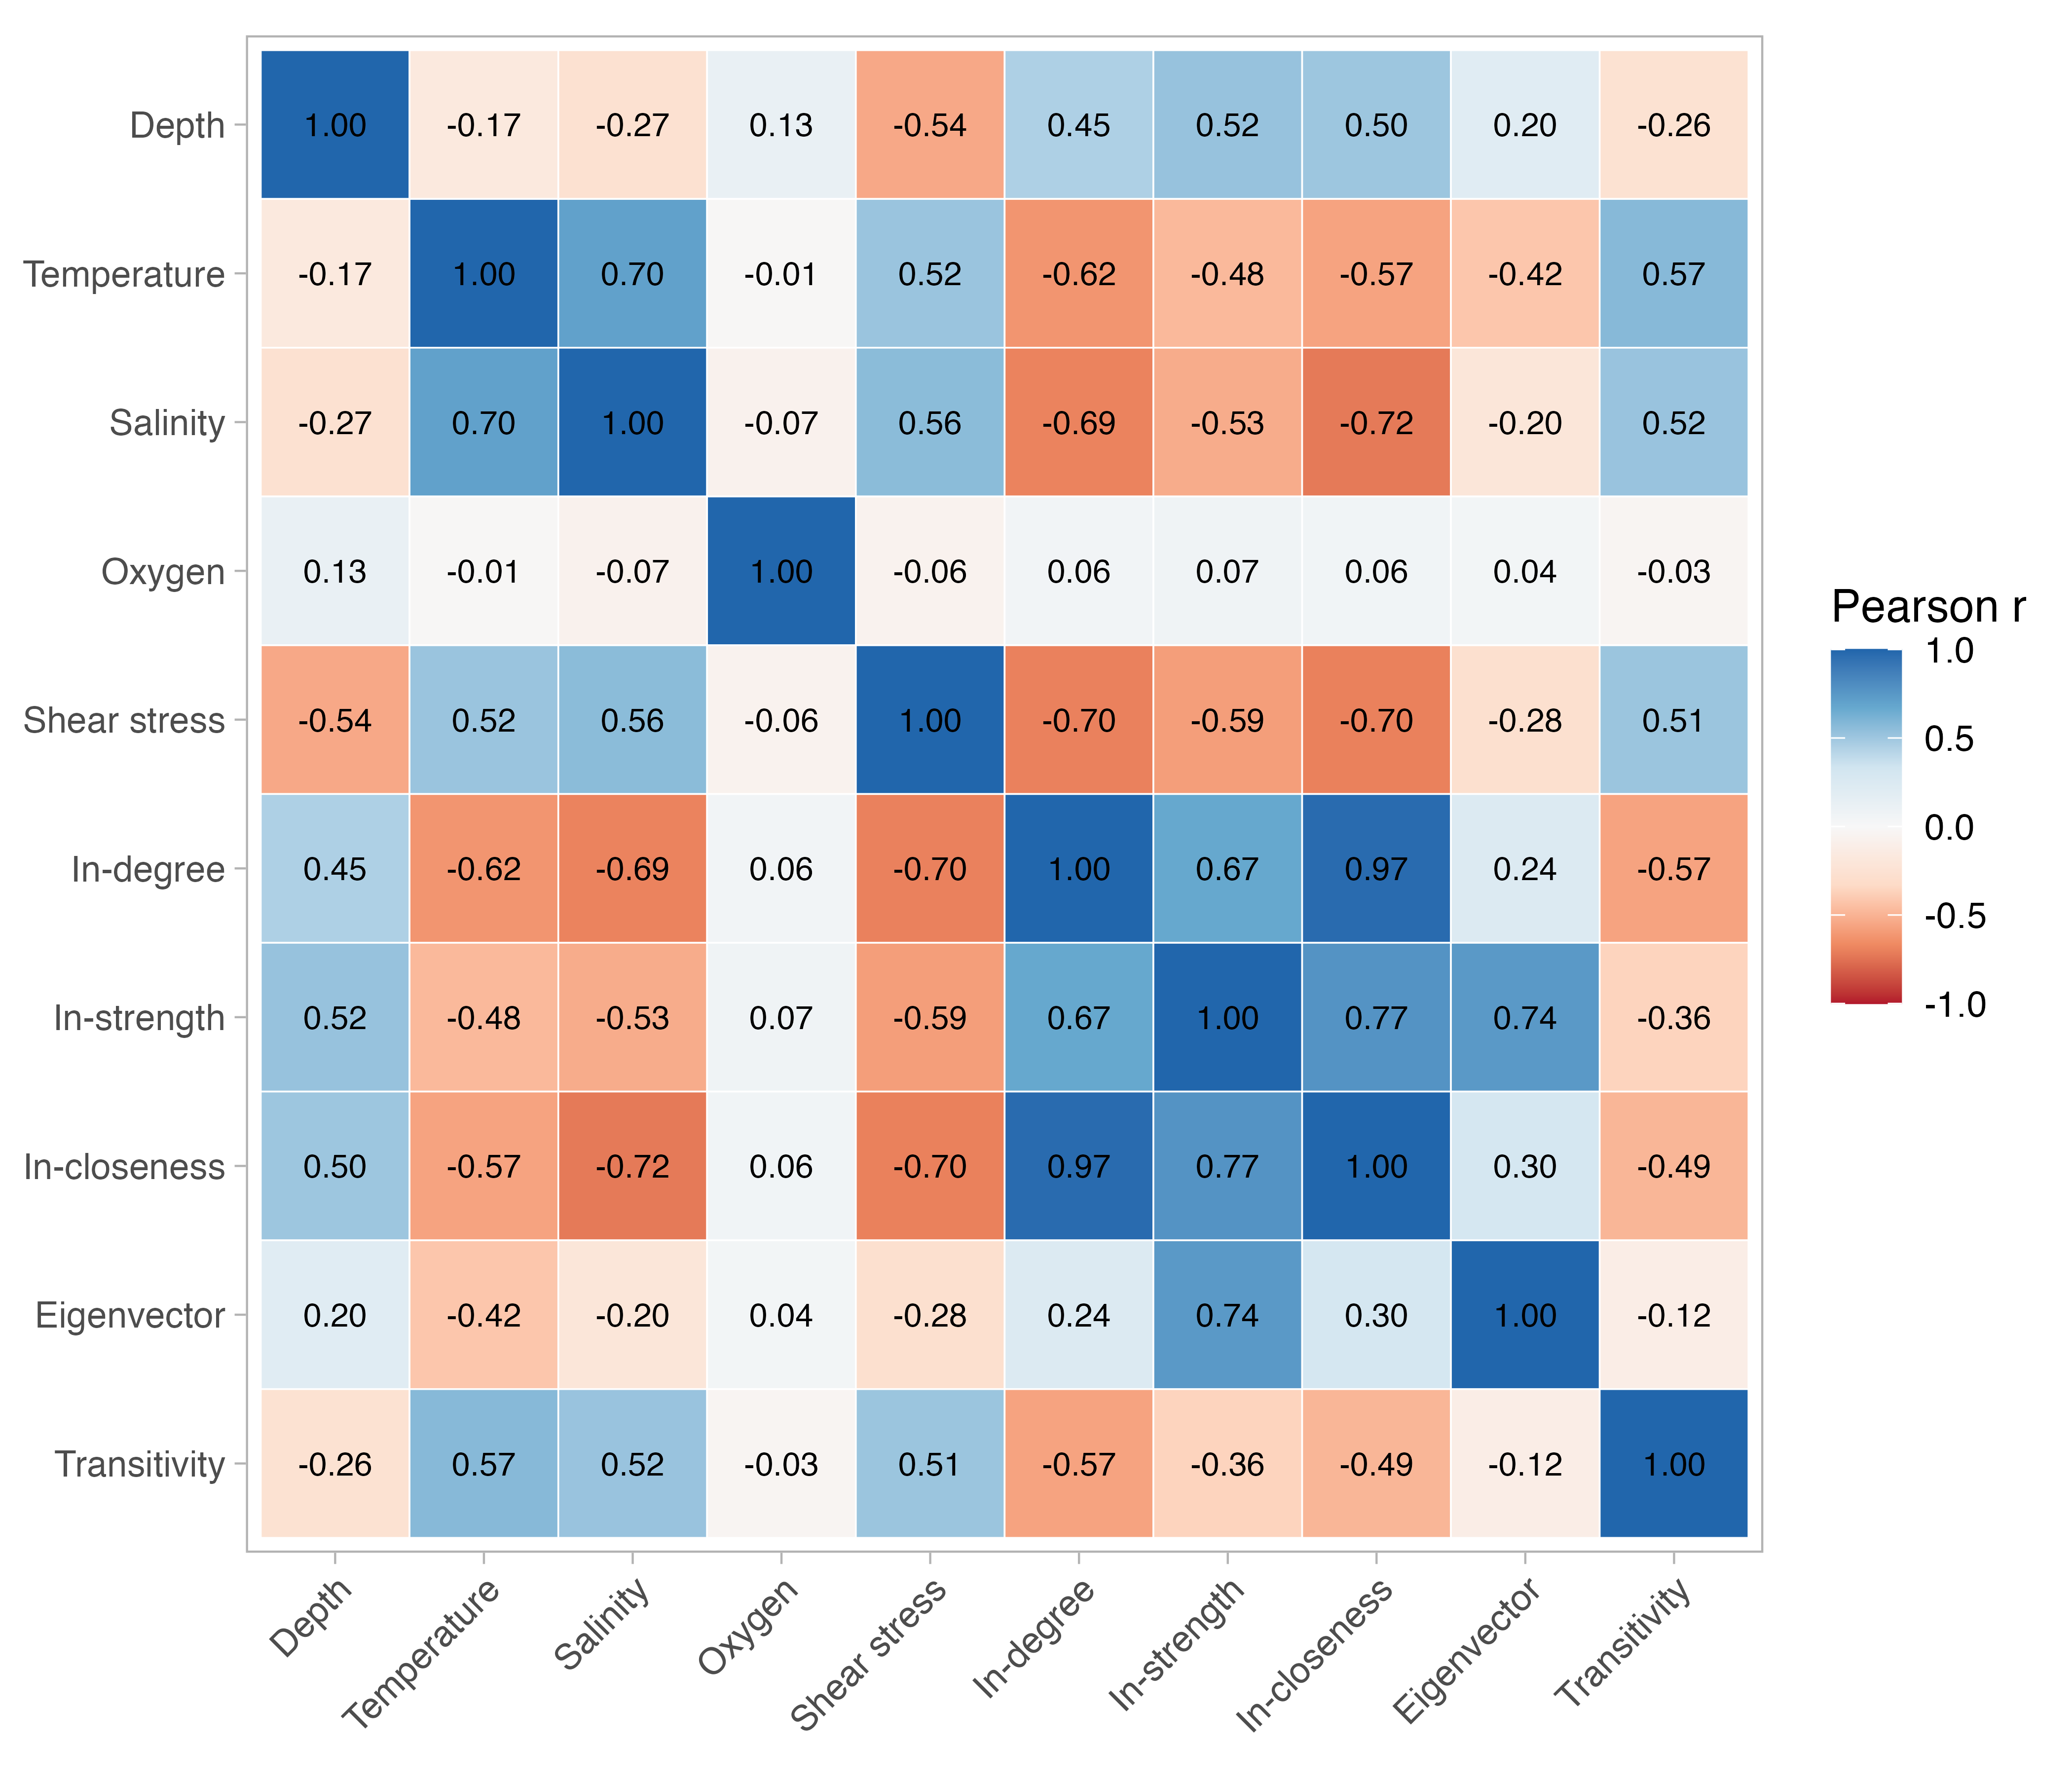
\includegraphics[width=0.7\textwidth]{figS3_correlation.png}
   % \caption{\rev{Pearson correlation among the five environmental predictors and five connectivity metrics.}}
    %\label{fig:conn_environment}
%\end{figure}
%\FloatBarrier
%\clearpage

%\begin{figure}[htb]
 %   \centering
  %  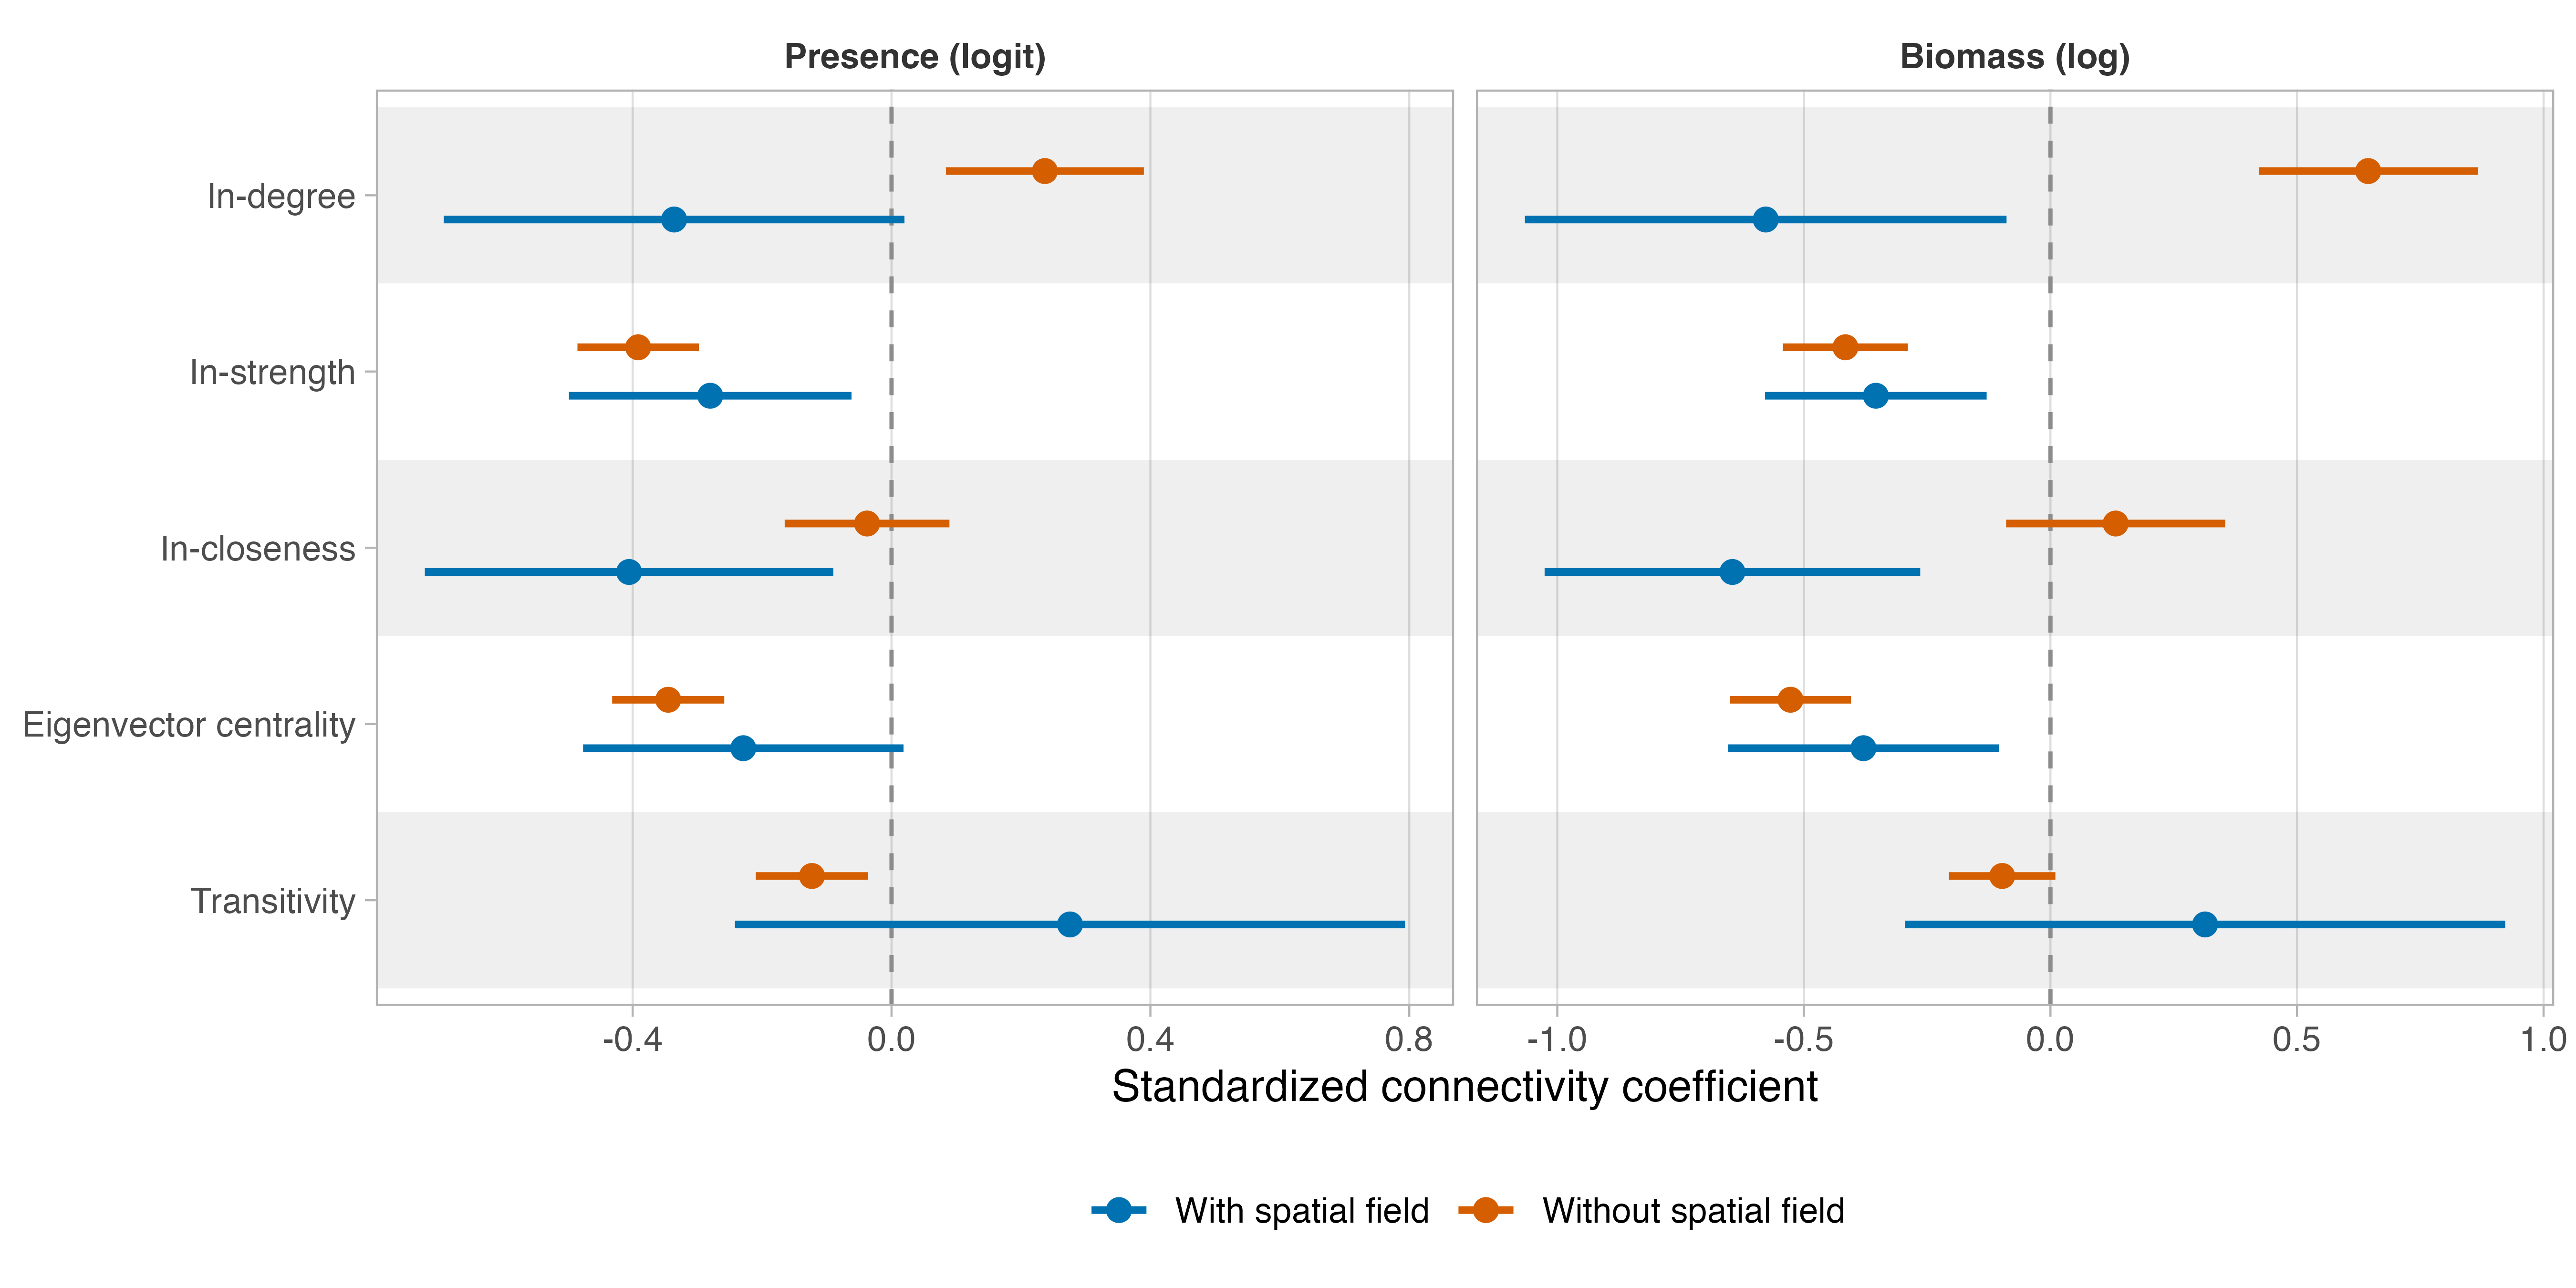
\includegraphics[width=0.95\textwidth]{figS4_space_confounding.png}
   % \caption{Connectivity coefficients estimated with and without the spatial random field, for each of the five connectivity metrics and both responses.}
    %\label{fig:space_confounding}
%\end{figure}
%\FloatBarrier
%\clearpage

%\begin{figure}[htb]
 %   \centering
  %  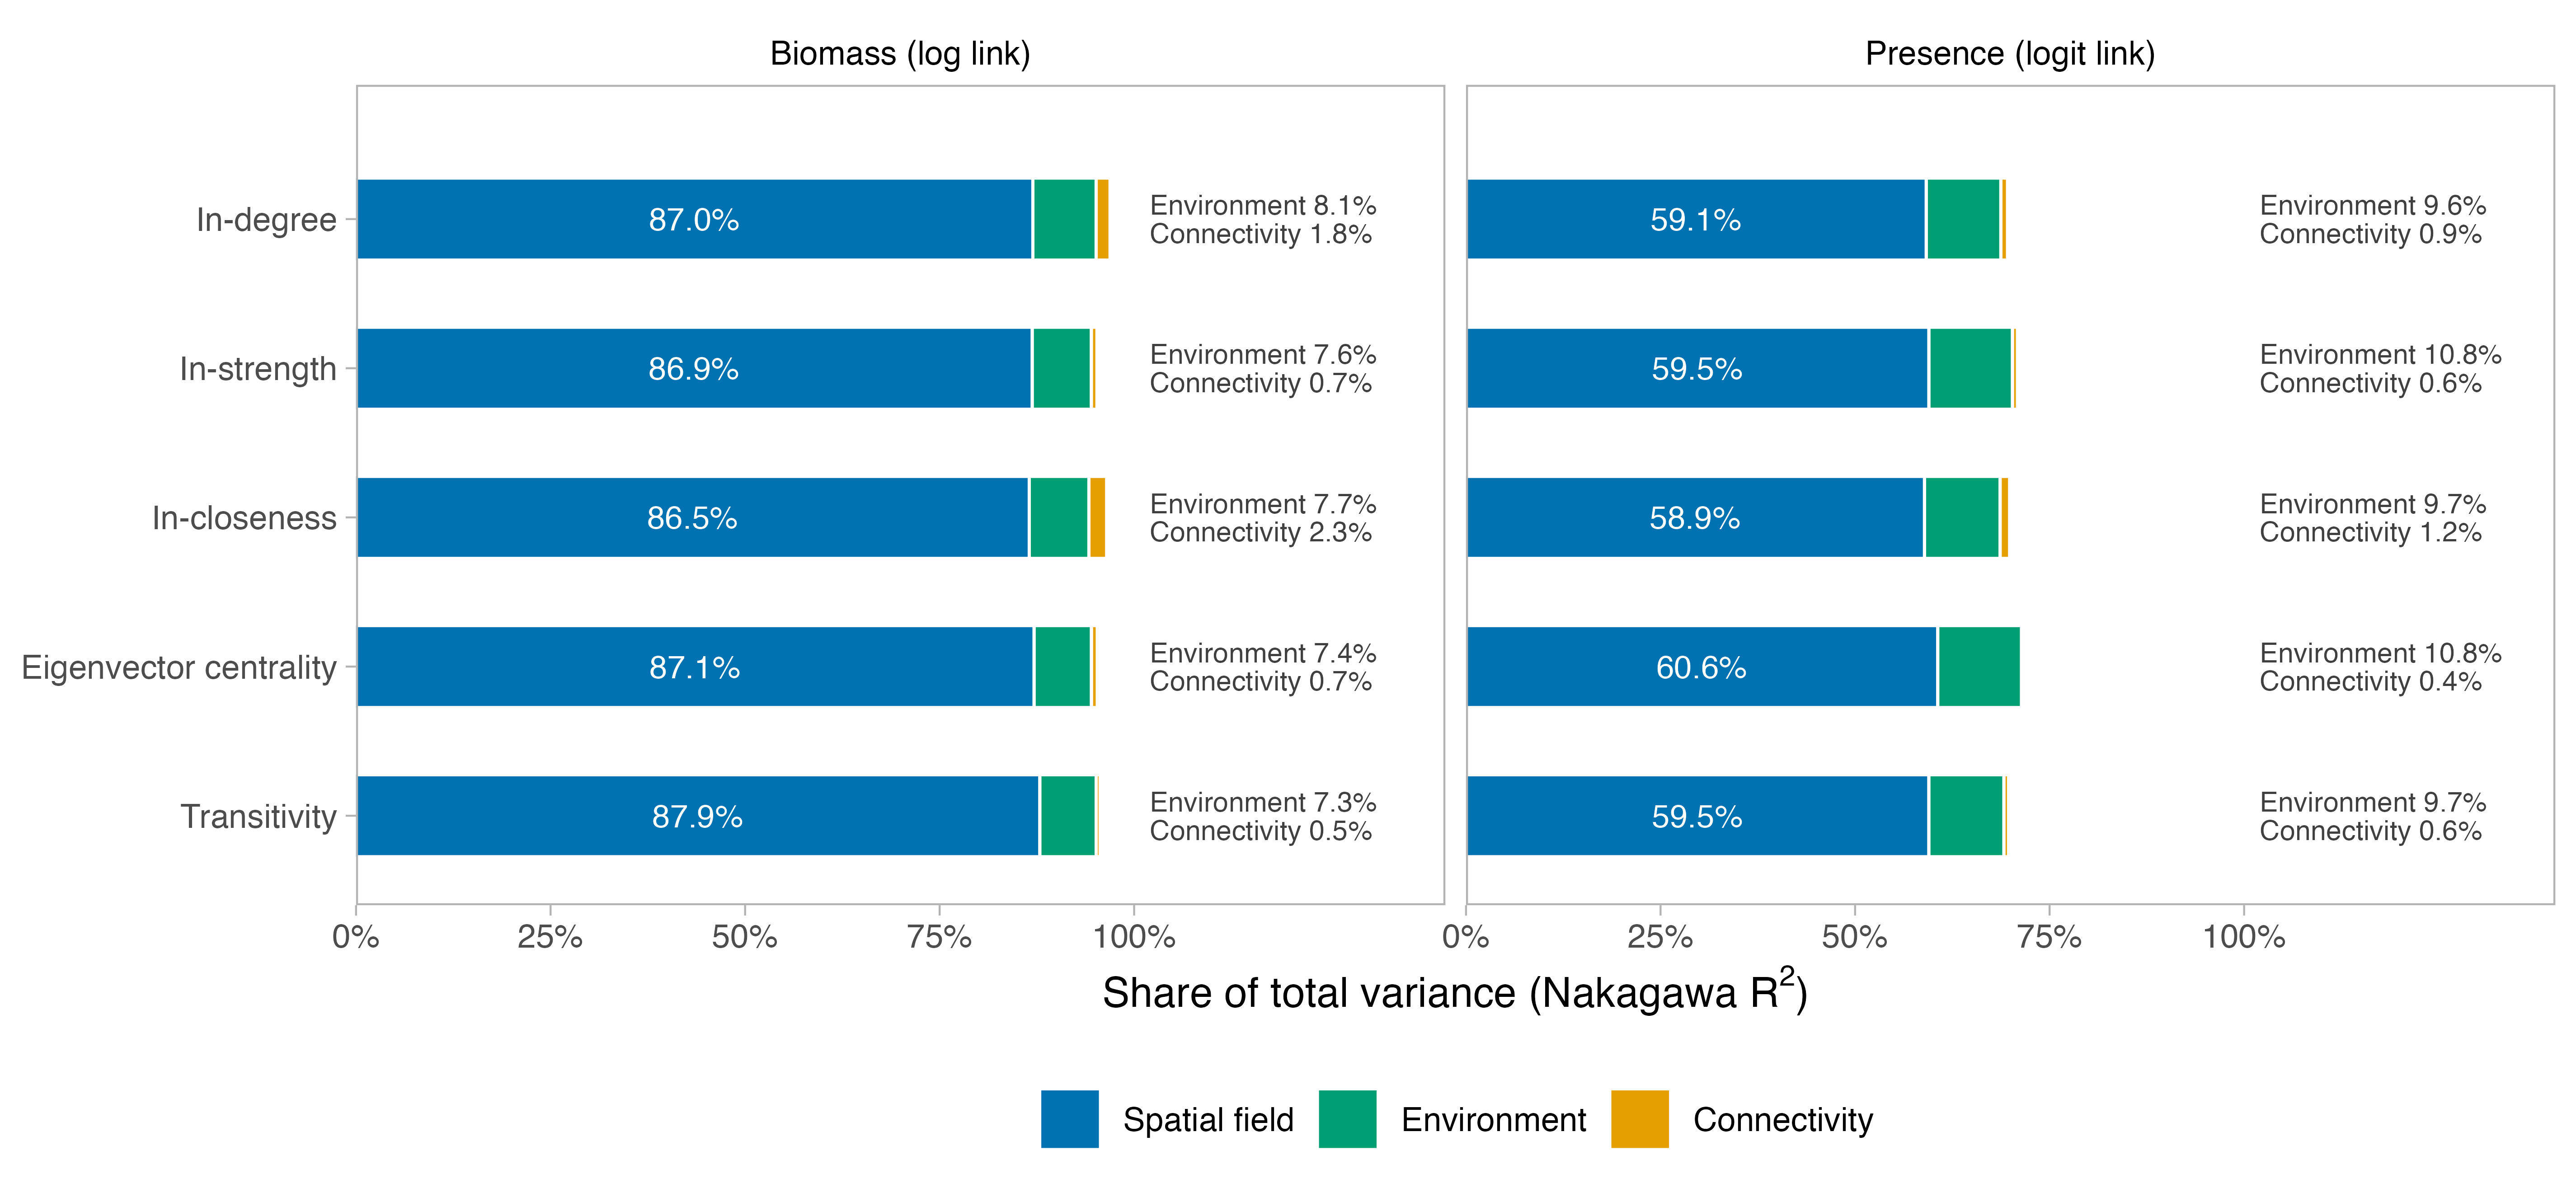
\includegraphics[width=0.95\textwidth]{figS5_variance_metrics.png}
   % \caption{\rev{Variance partitioning of the full model (spatial field included) using each of the five connectivity metrics in turn, both responses. Percentages indicate the share of total variance attributed to each model component.}}
    %\label{fig:variance_metrics}
%\end{figure}
%\FloatBarrier
%\clearpage

%\begin{figure}[htb]
 %   \centering
  %  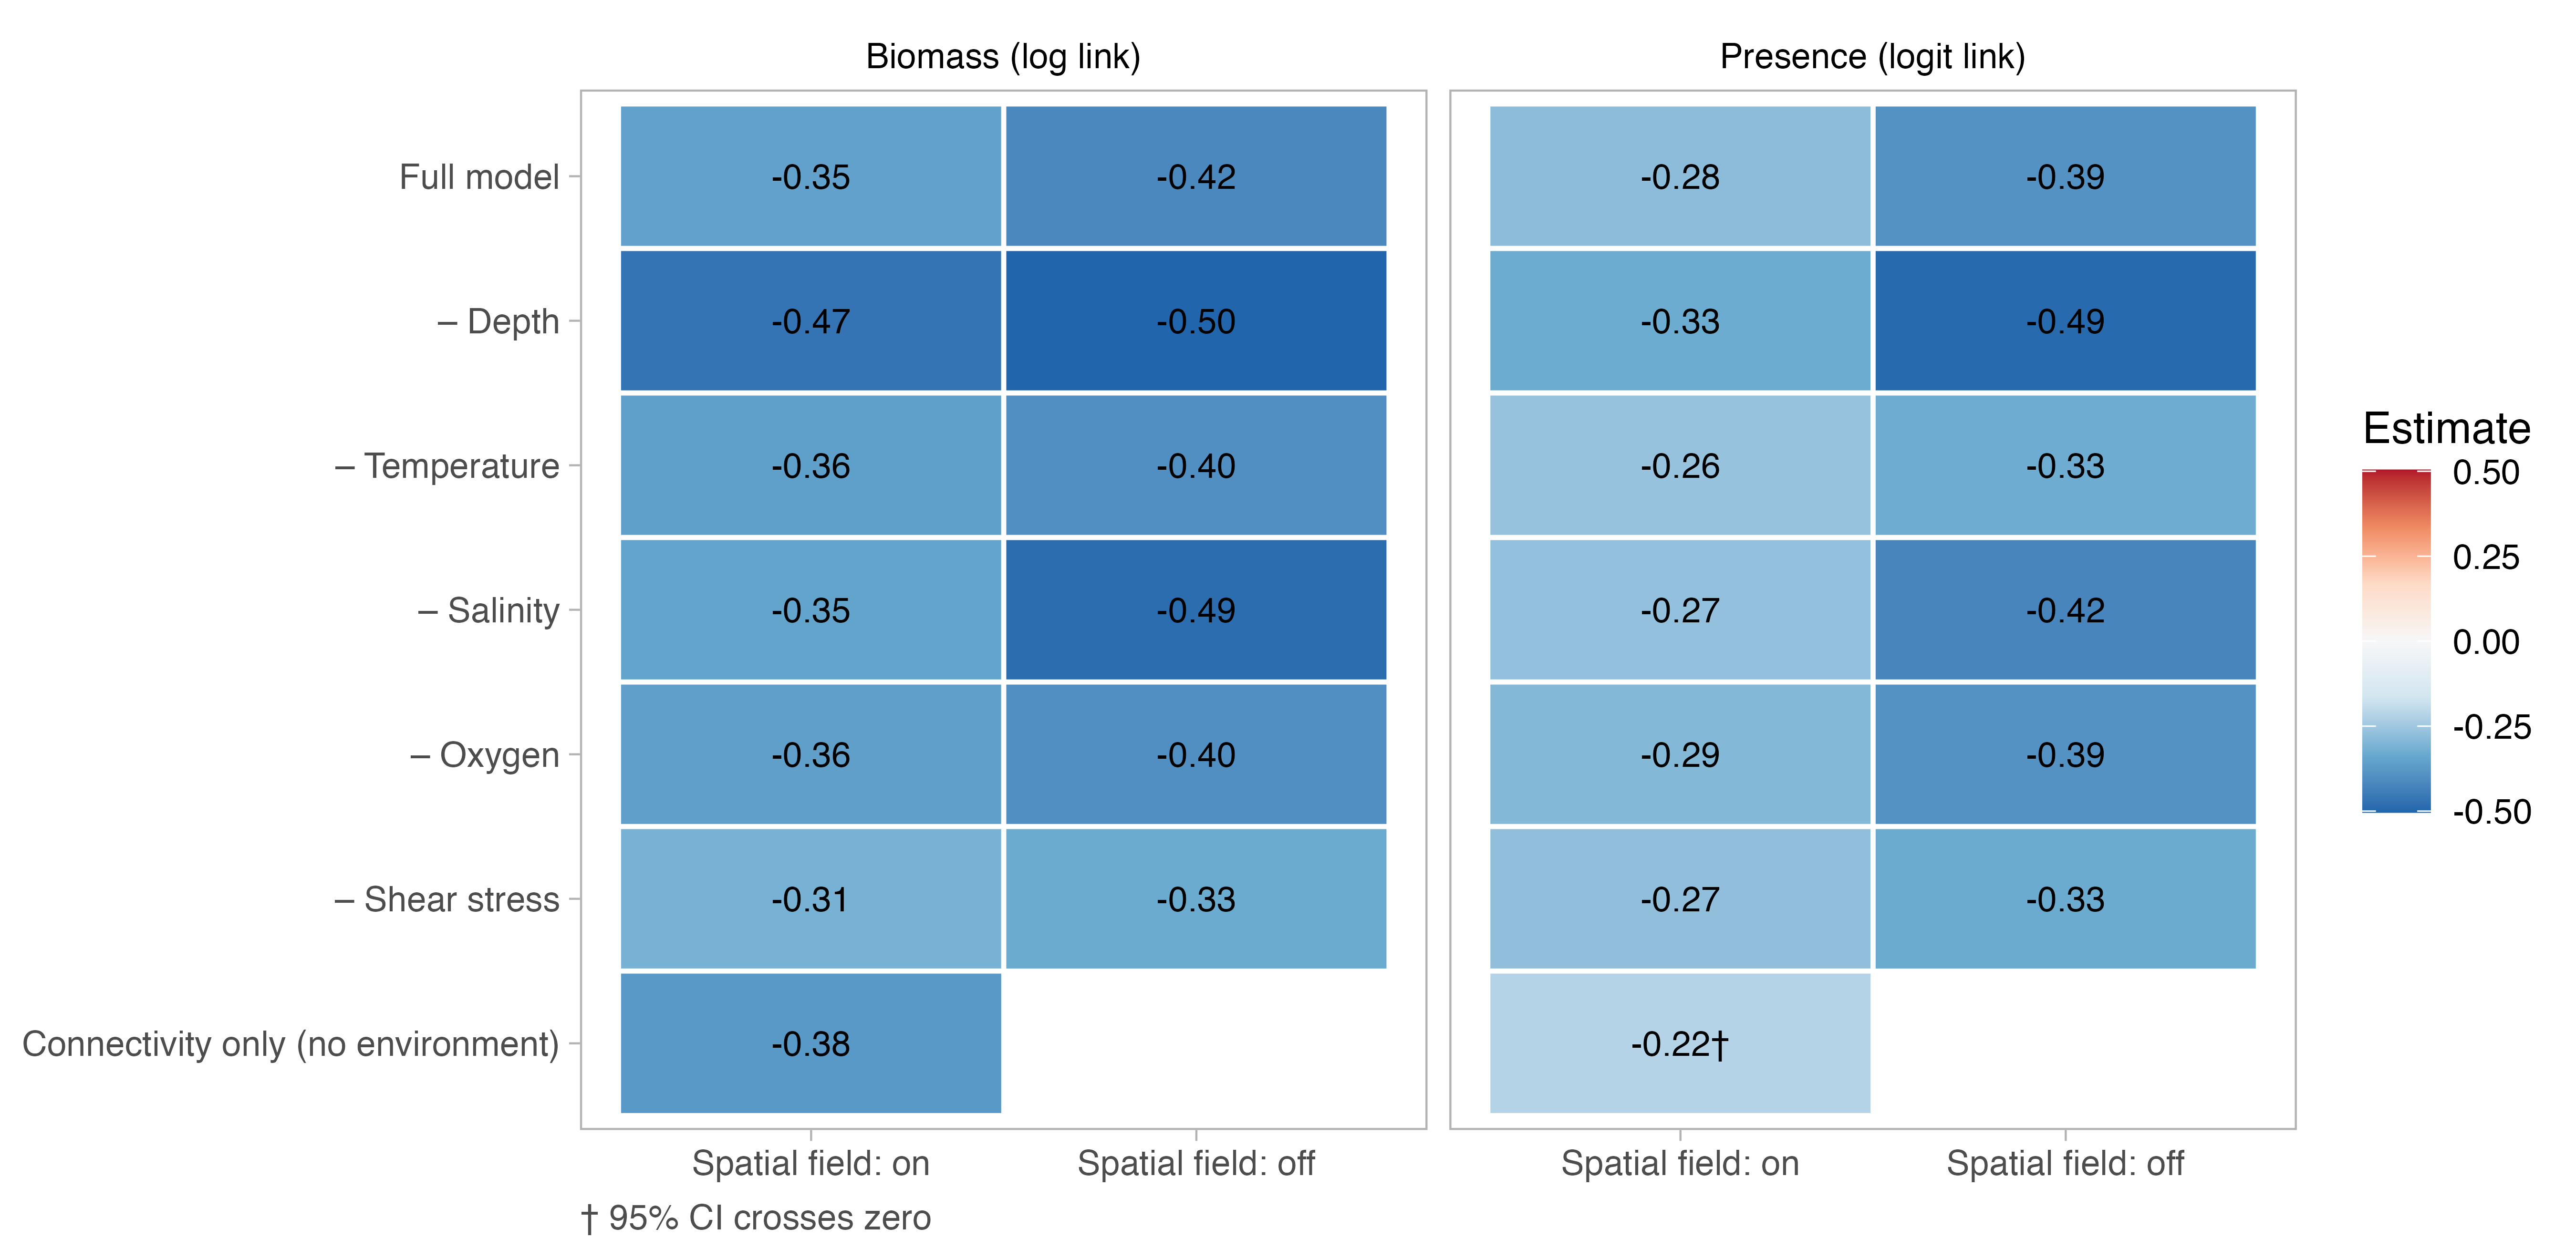
\includegraphics[width=0.95\textwidth]{figS6_coeff_stability.png}
   % \caption{\rev{Stability of the in-strength coefficient (both responses) across the full model, the full model with one environmental predictor dropped at a time, and connectivity alone, with and without the spatial field. A dagger marks a cell whose 95\% CI crosses zero; connectivity alone was fitted with the spatial field only.}}
    %\label{fig:loo_stability}
%\end{figure}
%\FloatBarrier
%\clearpage

%\begin{figure}[htb]
 %   \centering
  %  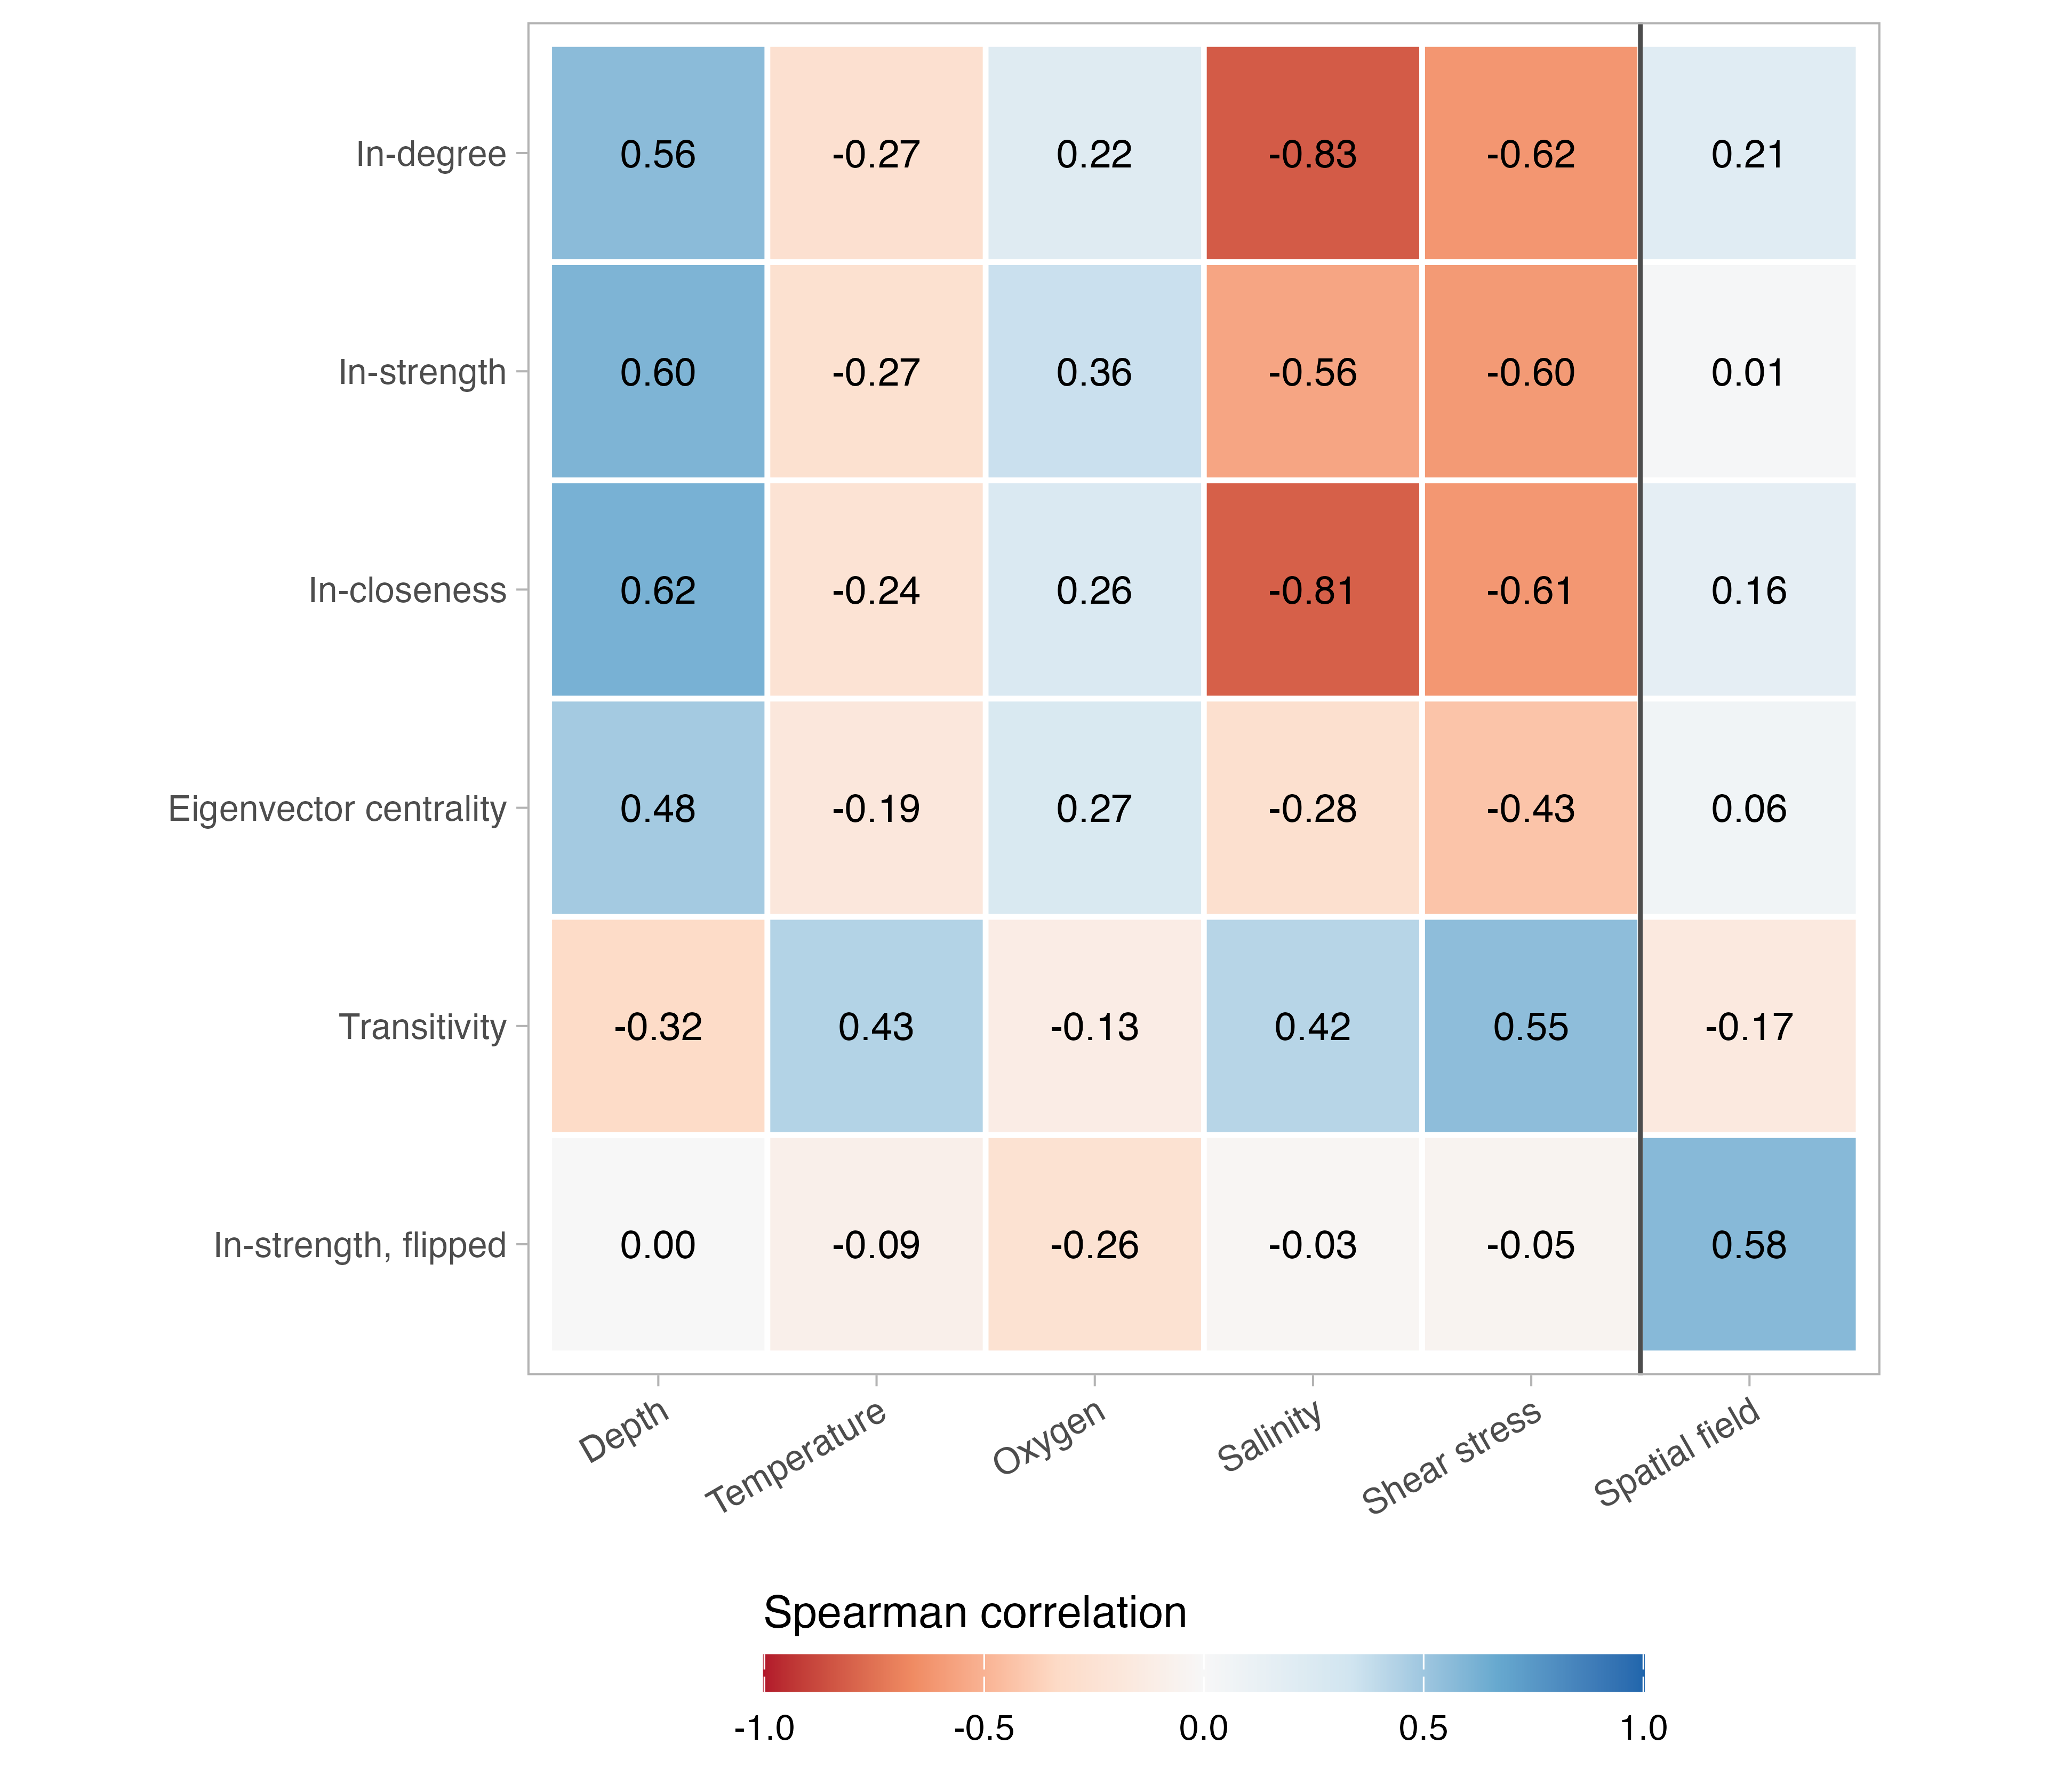
\includegraphics[width=0.7\textwidth]{figS7_connectivity_environment.png}
   % \caption{\rev{Spearman correlation, at the survey stations, between each connectivity metric (including flipped in-strength) and the five environmental predictors and the spatial random field of the Space + Environment biomass model.}}
    %\label{fig:conn_spatial}
%\end{figure}
%\FloatBarrier
%\clearpage





\end{document}
